\ExerciseGroupsStart
\ExerciseSection

\begin{enumerate}
\def\labelenumi{\arabic{enumi})}
\item
  设 G 是 \(R^{n}\) 中秩为 p 的离散子群，\((a_{i})_{1\leqslant i\leqslant p}\) 是 G 中 p 个点组成的一个自由系。第 1 号定理 1 的证明表明：G 是由 p 个点 \(d^{-1}a_{i}\) （d 为某个整数）所生成的群的一个子群。试不利用定理 1 证明：存在 G 中 p 个点组成的一个自由系 \(b_{i}=\sum_{j=1}^{p}b_{ij}a_{j}\)，使得若 \(x_{i}=\sum_{j=1}^{p}x_{ij}a_{j}\quad(\mathrm{I}\leqslant i\leqslant p)\) 是 G 中 p 个点组成的任意自由系，就有 \(|\det(x_{ij})|\geqslant|\det(b_{ij})|>0\) 。进而通过证明诸 \(b_{i}\) 生成 G，给出定理 1 的一个不依赖于不变因子理论的证明。（用反证法论证：若 \(z=\sum_{i=1}^{p}z_{i}b_{i}\in G\) 且诸 \(z_{i}\) 中有一个不是整数，则存在点 \(u=\sum_{i=1}^{p}u_{i}b_{i}\) 属于由 z 与诸 \(b_{i}\) 生成的群，使得对某个指标 i 有 \(o<u_{i}<1\) ，由此得出矛盾。）
\item
  设 G 是 \(R^{n}\) 的一个离散子群。若 G 是两个子群 H 与 K 的直和，则由 H 与 K 生成的向量子空间的交仅由 o 组成，因而 G 的秩等于 H 与 K 的秩之和（注意，对 \(R^{n}\) 的每个离散子群 G，由 G 生成的 \(R^{n}\) 的向量子空间典范地同构于 \(G \otimes_{Z} R\) ）。
\item
  设 G 是 \(R^{n}\) 的一个离散子群。要使 G 的子群 H 是 G 的一个直和项，必须且只须 \(H = V \cap G\) ，其中 V 是 \(R^{n}\) 的一个向量子空间（必要性用习题 2；充分性则注意 H 也是 G 与由 H 生成的向量子空间之交）。
\item
  设 H 与 K 是 \(R^{n}\) 的两个离散子群，使得 \(H + K\) 是闭子群。证明 \(H + K\) 此时是离散的，并且 \(r(\mathrm{H}) + r(\mathrm{K}) = r(\mathrm{H} \cap \mathrm{K}) + r(\mathrm{H} + \mathrm{K})\) 。（设 V 是 \(R^{n}\) 中由 \(H \cap K\) 生成的向量子空间；利用习题 3，把 H 分解为 \(V \cap H\) 与一个离散群 \(H_{1}\) 的直和，把 K 分解为 \(V \cap K\) 与一个离散群 \(K_{1}\) 的直和；然后证明和 \(H_{1} + K_{1}\) 是直和，并利用习题 2。）
\item
  设 G、\(G'\) 是 \(R^{n}\) 的两个闭子群，满足 \(G' \subset G\) ，又设 V（相应地 \(V'\) ）是包含在 G（相应地 \(G'\) ）中的最大向量子空间。证明存在一个与 V 互补的向量子空间 W，使得 G 是 V 与离散群 \(K = W \cap G\) 的直和，并且 \(G'\) 是 \(V \cap G'\) 与 \(K \cap G' = W \cap G'\) 的直和。（若 U 是与 \(V'\) 互补的向量子空间，用习题 3 证明离散群 \(U \cap G'\) 是 \(U \cap V \cap G'\) 与一个离散群 \(K'\) 的直和，并取 W 为包含 \(K'\) 的一个向量子空间。）由此推出：
\end{enumerate}

\begin{enumerate}
\def\labelenumi{\alph{enumi})}
\tightlist
\item
  商群 \(G/G'\) 同构于形如
\end{enumerate}

\[
\mathbf {R} ^ {p} \times \mathbf {T} ^ {q} \times \mathbf {Z} ^ {r} \times \mathbf {F},
\]

的乘积群，其中 F 是有限交换群。

\begin{enumerate}
\def\labelenumi{\alph{enumi})}
\setcounter{enumi}{1}
\tightlist
\item
  形如 \(R^{p} \times T^{q} \times Z^{r} \times F\) （F 有限且交换）的群的每个闭子群和每个豪斯多夫商群都具有同样的形式。
\end{enumerate}

\begin{enumerate}
\def\labelenumi{\arabic{enumi})}
\setcounter{enumi}{5}
\tightlist
\item
  设 H 与 K 是 \(R^{n}\) 的两个闭子群，使得 \(H + K\) 是闭子群。
\end{enumerate}

\begin{enumerate}
\def\labelenumi{\alph{enumi})}
\item
  证明：若 V（相应地 W）是包含在 H（相应地 K）中的最大向量子空间，则 \(V + W\) 是包含在 G 中的最大向量子空间，因而 \(d(\mathrm{H}) + d(\mathrm{K}) = d(\mathrm{H} \cap \mathrm{K}) + d(\mathrm{H} + \mathrm{K})\) {[}注意 \(\mathrm{G}/(\mathrm{V} + \mathrm{W})\) 的有理秩有限，因而 G 不能包含一条不含于 \(V + W\) 中的直线{]}。
\item
  设 U 是与 \(V + W\) 互补的一个子空间，使得 G 是 \(V + W\) 与 \(M = G \cap U\) 的直和，并且 \(H \cap K\) 是 \((V + W) \cap (H \cap K)\) 与 \(L = H \cap K \cap U\) 的直和（习题 5）。设 \(H'\) （相应地 \(K'\) ）是 M 中由 H（相应地 K）的点在 G 分解为 \(V + W\) 与 M 的直和中的分量所组成的子群。证明 \(M = H' + K'\) ，并且 \(H' \cap K' = L\) 。
\item
  若令 \(H'' = H \cap (V + W)\) ，\(K'' = K \cap (V + W)\) ，证明 \(r(H'') + r(K'') = r(H'' \cap K'') + r(H'' + K'')\) （化归为 \(V \cap W = \{o\}\) 的情形，并证明此时 \(H'' \cap K''\) 是 \(V \cap K''\) 与 \(W \cap H''\) 的直和。
\end{enumerate}

\(d\) ) 证明

\[
r (\mathrm{H}) + r (\mathrm{K}) = r (\mathrm{H} \cap \mathrm{K}) + r (\mathrm{H} + \mathrm{K})
\]

{[}利用 c) 与习题 4，注意 \(r(\mathbf{H}) = r(\mathbf{H}') + r(\mathbf{H}'')\) 以及 \(r(\mathbf{K}) = r(\mathbf{K}') + r(\mathbf{K}'' )\) {]}。

\begin{enumerate}
\def\labelenumi{\arabic{enumi})}
\setcounter{enumi}{6}
\item
  设 G 是 \(R^{n}\) 的一个闭子群，H 是 G 的一个闭子群。则 G 是 H 与另一个闭子群 K 的直和，当且仅当 H 是 G 与某个向量子空间之交。（必要性用习题 5；为证充分性，对 G 与 H 适当地应用第 2 号的定理 2，并利用习题 3）。
\item
  \begin{enumerate}
  \def\labelenumii{\alph{enumii})}
  \tightlist
  \item
    设 H、K 是 \(R^{n}\) 的两个闭子群。证明：若 \(r(\mathrm{H}) + r(\mathrm{K})\) 等于 \(r(\mathrm{H} \cap \mathrm{K}) + r(\mathrm{H} + \mathrm{K})\) ，则 \(H + K\) 在 \(R^{n}\) 中是闭的。{[}利用习题 7 与所给假设，化归为 H、K 与 \(H \cap K\) 都生成同一向量子空间的情形；若 V（相应地 W）表示包含在 H（相应地 K）中的最大子空间，则借助习题 5 证明 V 由 \(V \cap K\) 生成，W 由 \(W \cap H\) 生成；最后利用习题 7，把 \(H \cap K\) 分解为 \(H \cap K \cap (V + W)\) 与一个离散群的直和。{]}
  \end{enumerate}
\end{enumerate}

\begin{enumerate}
\def\labelenumi{\alph{enumi})}
\setcounter{enumi}{1}
\item
  由 a) 与习题 6 推出：若 H 与 K 是 \(R^{n}\) 的两个闭子群，使得 \(H + K\) 是闭子群，则 \(H^{*} + K^{*}\) 也是闭子群。
\item
  由 b) 推出：若 H 与 K 是 \(R^{n}\) 的两个闭子群，使得 \(d(\mathrm{H}) + d(\mathrm{K}) = d(\mathrm{H} \cap \mathrm{K}) + d(\overline{\mathrm{H} + \mathrm{K}})\) ，则子群 \(H + K\) 是闭的。
\end{enumerate}

\begin{enumerate}
\def\labelenumi{\arabic{enumi})}
\setcounter{enumi}{8}
\item
  设 G 是 \(R^{n}\) 的一个子群，不必是闭的，秩为 p，又设 V 是包含在 \(\overline{G}\) 中的最大向量子空间。若 V 的维数 \(q \leqslant p\) ，证明 G 是 \(V \cap G\) 与一个秩为 p - q 的离散子群的直和，该离散子群包含在与 V 互补的一个向量子空间中{[}注意，对每个 \(x \in \overline{G}\) ，\((x + V) \cap G\) 在线性簇 \(x + V\) 中稠密{]}。
\item
  设 \(a\) 是一个实数，\(n\) 是一个 \(>0\) 的整数，考虑数 \(x_{k} = ka - [ka] \in [0, \mathrm{I}[(\mathrm{I} \leqslant k \leqslant n + \mathrm{I})\) 。若 \(\mathbf{I}_h\) 表示区间
\end{enumerate}

\[
\left[ \frac {h - \mathrm{I}}{n}, \frac {h}{n} \right] \quad (\mathrm{I} \leqslant h \leqslant n),
\]

证明存在两个不同的指标 \(k, k'\) ，使得 \(x_k\) 与 \(x_{k'}\) 属于同一个区间 \(I_h\) （对某个适当的 \(h\) 值）。由此推出存在两个整数 \(p, q\) ，使得 \(1 \leqslant p \leqslant n\) 且 \(|pa - q| \leqslant 1 / n\) 。

\begin{enumerate}
\def\labelenumi{\Roman{enumi})}
\setcounter{enumi}{1}
\tightlist
\item
  设 \(\boldsymbol{a}_i = (a_{ij})\) （ \(1 \leqslant i \leqslant m\) ，\(1 \leqslant j \leqslant n\) ）是 \(m\) 个属于 \(\mathbf{R}^n\) 的点，又设 \(q\) 是一个 \(>0\) 的整数。对每个形如 \(\boldsymbol{k} = (k_i)\) （ \(1 \leqslant i \leqslant m\) ）的点，它属于 \(\mathbf{R}^m\) 、具有整数坐标（不全为零）且满足不等式 \(0 \leqslant k_i \leqslant q\) ；对这样的点，考虑点 \(x_k = (x_{j,k})\) （ \(1 \leqslant j \leqslant n\) ），它属于 \(\mathbf{R}^n\) ，其所有坐标都属于 {[}o, i{[} ，并且它模 \(Z^n\) 同余于 \(\sum_{i=1}^{m} k_i a_i\) ，即坐标为
\end{enumerate}

\[
x _ {j, k} = \sum_ {i = 1} ^ {m} k _ {i} a _ {i j} - \left[ \sum_ {i = 1} ^ {m} k _ {i} a _ {i j} \right].
\]

  的点。若 \(p\) 是使 \(q + 1 \geqslant p^{n/m}\) 的最小整数，证明存在两个不同的点 \(k, k'\) ，使得 \(x_k\) 与 \(x_{k'}\) 都属于同一个棱长为 \(1/p\) 的立方体（方法与习题 10 相同）。由此推出：存在 \(m\) 个不全为零的整数 \(p_i\) 以及 \(n\) 个整数 \(r_j\) （ \(1 \leqslant j \leqslant n\) ），使得 \(0 \leqslant p_i \leqslant q\) 对 \(1 \leqslant i \leqslant m\) 成立，并且

\[
\left| \sum_ {i = 1} ^ {m} p _ {i} a _ {i j} - r _ {j} \right| \leqslant \frac {\mathrm{I}}{p} \quad (\mathrm{I} \leqslant j \leqslant n).
\]

利用这一结果，给出第 1 号命题 2（“抽屉原理”）的另一个证明。

\begin{enumerate}
\def\labelenumi{\arabic{enumi})}
\setcounter{enumi}{11}
\tightlist
\item
  对每一对实数 \((\theta, \beta)\) ，存在无穷多个整数三元组 \((p, q, r)\) ，使得 \(r > 0\) ，\(|q| \leqslant \frac{1}{2} r\) ，并且
\end{enumerate}

\[
- \frac {\mathrm{I}}{r} <   \theta q + p - \beta <   \frac {\mathrm{I}}{r}.
\]

{[}若 \(m, n\) 是使 \(|n\theta - m| < 1/n\) 的两个整数（习题 10），取 \(r = n\) ，并选取 \(p, q\) 使得 \(pn + qm\) 与 \(n\beta\) 之差小于 \(1/2\) 。{]}

\begin{enumerate}
\def\labelenumi{\arabic{enumi})}
\setcounter{enumi}{12}
\tightlist
\item
  \(n\) 阶法里数列（\(n\) 为 \(>0\) 的整数）是集 \(F_n\) ，它由既约形式的有理数 \(p/q\) （满足 \(0 \leqslant p \leqslant q \leqslant n\) ）组成，按递增次序排列（也就是说，法里数列是一个序列）。
\end{enumerate}

\begin{enumerate}
\def\labelenumi{\alph{enumi})}
\item
  证明：若两个有理数 \(r = p / q\) 、\(r' = p' / q'\) 满足 \(p'q - pq' = \pm 1\) ，则每一对整数 \((p'', q'')\) 都可以表示成形式 \(p'' = px + p'y\) ，\(q'' = qx + q'y\) ，其中 \(x\) 与 \(y\) 是整数。分数 \(p'' / q''\) 属于以 \(r\) 与 \(r'\) 为端点的闭区间，当且仅当 \(x\) 与 \(y\) 同号。
\item
  由 a) 推出：若 \(r = p / q\) 与 \(r' = p' / q'\) 是 {[}0, 1{]} 中的两个有理数，满足 \(q > 0\) 、\(q' > 0\) 且 \(qp' - pq' = \pm 1\) ，则 \(r\) 与 \(r'\) 是数列 \(\mathbf{F}_n\) 中相邻的元素，其中 \(n = \max (q, q')\) 。此外，设 \(m\) 为使以 \(r\) 与 \(r'\) 为端点的开区间含有 \(\mathbf{F}_m\) 中一点的最小整数，则 \(m = q + q'\) ，并且在此区间中只有 \(\mathbf{F}_{q + q'}\) 的一个点，即分数 \((p + p') / (q + q')\) 。
\item
  反之，证明若 \(r\) 与 \(r'\) 是 \(\mathbf{F}_n\) 的两个相邻元素，则有 \(p'q - pq' = \pm 1\) （对 \(n\) 用归纳法）。
\item
  由 c) 推出：对每个实数 \(\theta \in [\mathrm{o},\mathrm{i}]\) 以及每个整数 \(n\geqslant \mathrm{i}\) ，至少存在一个既约形式的分数 \(p / q\) ，使得 \(\mathrm{i}\leqslant q\leqslant n\) 且 \(|\theta -p / q|\leqslant \mathrm{i} / (n + \mathrm{i})q\) （参看习题 10）。
\item
  若 \(p / q\) 是一个既约形式的分数，满足 \(|\theta - p / q| < 1 / q^2\) ，则 \(\theta\) 属于以法里数列 \(\mathbf{F}_q\) 中与 \(p / q\) 相邻的两项为端点的开区间。
\end{enumerate}

\begin{enumerate}
\def\labelenumi{\arabic{enumi})}
\setcounter{enumi}{13}
\tightlist
\item
  设 \(\varphi: \mathbf{R} \to \mathbf{T}\) 是典范同态；设 \(\theta\) 是 \(\mathbf{T}\) 中一个无限阶的元素，又设 \(\theta_0\) 是使 \(\varphi(\theta_0) = \theta\) 的（无理）实数。对每个整数 \(n > 0\) ，设 \(\mathbf{S}_n\) 是形如 \(k\theta\) 的元素（属于 \(\mathbf{T}\) ，且 \(\mathbf{i} \leqslant k \leqslant n\) ）所成的集，又对每个区间 \(\mathbf{I}\) （\(\mathbf{R}\) 的），设 \(\mathrm{N}(\mathbf{I}, n)\) 是集 \(\mathbf{I} \cap \overline{\varphi}^1(\mathbf{S}_n)\) 的元素个数。
\end{enumerate}

\begin{enumerate}
\def\labelenumi{\alph{enumi})}
\item
  若取 \(\mathbf{I} = [\mathrm{o},\theta_0[\) ，证明 \(\mathrm{N(I,n)} = [n\theta_0]\) {[}注意，此时 \(\mathrm{N(I,n)}\) 是如下整数对 \((x,y)\) 的个数：\(\mathrm{i}\leqslant y\leqslant n\) 且 \(x\leqslant y\theta_0 < x + \theta_0]\) 。
\item
  更一般地，若取 \(\mathbf{I} = [\mathrm{o}, m\theta_0[, m\) 为整数，则有 \(m. [(n - m)\theta_0] \leqslant \mathrm{N}(\mathrm{I}, n) \leqslant m. [n\theta_0]\) （同样的方法）。
\item
  由此推出：若 I 是任意区间，则数 \(\mathrm{N}(\mathrm{I}, n)/n\) 当 \(n \to +\infty\) 时趋于一个等于 I 的长度的极限。（先对形如 \([m\theta_{0} + a, m'\theta_{0} + a']\) 的 I 证明该结果，其中 \(m, m', a\) 与 \(a'\) 是整数，利用 b)；然后用形如 \(m\theta_{0} + a\) 的数逼近 I 的端点，过渡到一般情形。）{[}“序列 \((k\theta) \mod 1\) 的均分”。{]}
\end{enumerate}

* 15) 设 I 是 \(\mathbf{R}^n\) 中一个棱长为 \(2\pi\) 的闭立方体。把 I 的每个点 \(x = (x_i)\) 映为点 \(y = (y_j)\) （属于 \(\mathbf{R}^{n+1}\) ），使得

\[
\begin{array}{l} y _ {1} = \sin x _ {1} \\ y _ {2} = (2 + \cos x _ {1}) \sin x _ {2} \end{array}
\]

\[
y _ {p} = \left(2 ^ {p - 1} + \sum_ {k = 1} ^ {p - 1} 2 ^ {p - k - 1} \cos x _ {p - k} \cos x _ {p - k + 1} \dots \cos x _ {p - 1}\right) \sin x _ {p} \quad (2 \leqslant p \leqslant n)
\]

\[
y _ {n + 1} = \sum_ {k = 1} ^ {n - 1} 2 ^ {p - k - 1} \cos x _ {n - k} \cos x _ {n - k + 1} \dots \cos x _ {n}.
\]

 证明 I 在此映射下的像同胚于 \(T^{n}\) （对 n 用归纳法证明：注意 \(y_{p}\) 与 \(\sin x_{p}\) 当 \(2 \leqslant p \leqslant n\) 时同号）。若 n=2，这样定义的 \(R^{3}\) 的子集称为旋转环面。*

¶ 16) 设 G 是 \(\mathbf{R}^n\) 的一个子群，它包含一个紧连通子集 K，使得由 K 生成的仿射线性簇的维数是 \(p\) 。证明 G 包含一个维数为 \(p\) 的向量子空间。{[}对 \(n\) 用归纳法证明，并利用第六章 § 1 的习题 10 c)。{]}

\(\mathbb{J}\) 17) 设 \(\mathbf{E}\) 是乘积 \((\mathbf{Q}_p)^n\) ：它由 \(n\) 个都等于域 \(\mathbf{Q}_p\) （\(p\) 进数域）的因子组成（第三章，§ 6，习题 23），赋有由诸因子 \(\mathbf{Q}_p\) 的加法拓扑结构的乘积所成的拓扑群结构，以及它的 \(n\) 维向量空间结构（在域 \(\mathbf{Q}_p\) 上）。若 \(v\) 表示加法 \(p\) 进赋值（在 \(\mathbf{Q}_p\) 上），则令 \(|x|_p = p^{-v_p(x)}\) ，其中 \(x \neq 0\) 属于 \(\mathbf{Q}_p\) ，并令 \(|o|_p = 0\) ；又令 \(||x|| = \sup |x_i|_p\) （对一切 \(x = (x_i)_{1 \leqslant i \leqslant n} \in \mathbf{E}\) ）（参看第九章，§ 3，第 2 号与第 3 号）。

\begin{enumerate}
\def\labelenumi{\alph{enumi})}
\tightlist
\item
  子集 \(\mathbf{A}\) （\(\mathbf{E}\) 的）是相对紧的，当且仅当
\end{enumerate}

\[
\sup _ {\mathbf {x} \in \mathbf {A}} | | \mathbf {x} | | <   + \infty .
\]

{[}注意 \(v_{p}\) 是 \(\mathbf{Q}_p\) 到 \(\mathbf{Z}\) （带离散拓扑）中的连续映射。{]}

\begin{enumerate}
\def\labelenumi{\alph{enumi})}
\setcounter{enumi}{1}
\item
  若 \(\mathbf{G}\) 是 \(\mathbf{E}\) 的一个闭子群，则 \(\mathbf{G}\) 是环 \(\mathbf{Z}_p\) （\(p\) 进整数环）上的一个拓扑模（若 \(\boldsymbol{x} \in \mathbf{G}\) ，则有 \(n\boldsymbol{x} \in \mathbf{G}\) （对一切 \(n \in \mathbf{Z}\) ），而 \(\mathbf{Z}\) 在 \(\mathbf{Z}_p\) 中稠密）。
\item
  若 K 是 E 的一个紧子群，则存在 E 的 \(m \leqslant n\) 个点 \(a_{i}\) （ \(i \leqslant i \leqslant m\) ）组成的一个自由系，使得 K 是 m 个群 \(Z_{p}.a_{i}\) 的直和。{[}利用 a) 证明：若 \((\boldsymbol{e}_{j})_{1 \leqslant j \leqslant n}\) 是 E 的标准基，则存在一个整数 \(k \in Z\) ，使得 K 包含在 n 个群 \(Z_{p}.p^{k}\boldsymbol{e}_{j}\) 的直和中；然后应用主理想环上的模的理论。{]}
\item
  若 G 是 E 的一个闭（但非紧）子群，则 G 包含一个一维向量子空间，即 \(Q_{p} \cdot a\) ，其中 \(a \neq 0\) 。{[}设 C 是由所有点 \(x \in E\) （满足 \(\|x\| = 1\) ）组成的 E 的紧子集；证明 \(G \cap C\) 包含一个点列 \((\boldsymbol{x}_{r})_{r \in \mathbb{N}}\) ，使得 \(p^{-r}x_{r} \in G\) ，并取 a 为该序列的一个聚点。{]}
\item
  设 G 是 E 的一个闭子群，V 是包含在 G 中的最大向量子空间，W 是与 V 互补的一个向量子空间；证明 \(W \cap G\) 是紧的，并且 G 是 V 与 \(W \cap G\) 的直和（按第 2 号定理 2 的方式论证）。
\end{enumerate}

\(f)\) 给定一个子群 \(\mathbf{G}\) （\(\mathbf{E}\) 的），用 \(\mathbf{G}^*\) 表示所有 \(\boldsymbol{u} = (u_i) \in \mathbf{E}\) 中使得

\[
(u | x) = \sum_ {i = 1} ^ {n} u _ {i} x _ {i}
\]

属于 \(\mathbf{Z}_p\) （对所有 \(x = (x_i) \in \mathbf{G}\) ）者所成的集。证明 \(\mathbf{G}^*\) 在 \(\mathbf{E}\) 中是闭的，\((\overline{\mathbf{G}})^* = \mathbf{G}^*\) ，并且 \((\mathbf{G}^*)^* = \overline{\mathbf{G}}\) 。

\begin{enumerate}
\def\labelenumi{\alph{enumi})}
\setcounter{enumi}{6}
\tightlist
\item
  对 E 的闭子群，叙述并证明习题 2 至 8（包括 8 在内）的类似命题。特别地，形如
\end{enumerate}

\[
(\mathbf {Q} _ {p}) ^ {r} \times (\mathbf {Q} _ {p} / \mathbf {Z} _ {p}) ^ {s} \times (\mathbf {Z} _ {p}) ^ {t} \times \mathbf {F}
\]

（其中 F 是有限个 p 幂阶循环群的乘积）的群的每个闭子群和每个豪斯多夫商群都是同样形式的群。

\ExerciseSection

\begin{enumerate}
\def\labelenumi{\arabic{enumi})}
\tightlist
\item
  设 \(\varphi\) 是 \(\mathbf{R}^n\) 到 \(\mathbf{T}^n\) 上的典范同态，\(u\) 是 \(\mathbf{R}^m\) 到 \(\mathbf{R}^n\) 中的一个线性映射。要使 \(\varphi \circ u\) 是 \(\mathbf{R}^m\) 到 \(\mathbf{T}^n\) 中的一个严格态射，必须且只须下列条件之一成立：
\end{enumerate}

\begin{enumerate}
\def\labelenumi{\alph{enumi})}
\item
  \(\overline{u}^1 (\mathbf{Z}^n)\) 的秩为 \(m\) ；或者
\item
  \(u(\mathbf{R}^m)\cap \mathbf{Z}^n\) 的秩等于 \(u(\mathbf{R}^m)\) 的维数。
\end{enumerate}

\begin{enumerate}
\def\labelenumi{\arabic{enumi})}
\setcounter{enumi}{1}
\item
  证明：从 p 进数的加法拓扑群 \(Q_{p}\) （第三章，§ 6，习题 23 及其后各题）到加法群 R 中的连续同态只有零映射。
\item
  每个 \(p\) 进数 \(x\) （习题 2）都可以写成形式 \(\sum_{-\infty}^{+\infty} \alpha_k p^k\) ，其中诸 \(\alpha_k\) 是有理整数，且指标 \(k < 0\) 的那些除对指标 \(k\) 的有限多个值外全为零。此外，若 \(\sum_{-\infty}^{+\infty} \alpha_k p^k = \sum_{-\infty}^{+\infty} \beta_k p^k\) ，则有理数 \(\sum_{-\infty}^{-1} \alpha_k p^k\) 与 \(\sum_{-\infty}^{-1} \beta_k p^k\) 模 1 同余。设 \(\varphi_p(x)\) 是有理数 \(\sum_{-\infty}^{-1} \alpha_k p^k\) 的模 1 类。\\
\end{enumerate}

\begin{enumerate}
\def\labelenumi{\alph{enumi})}
\tightlist
\item
  证明 \(\varphi_p\) 是拓扑群 \(\mathbf{Q}_p\) 到 \(\mathbf{T}\) 中的一个连续同态，并且对每个连续同态 \(f\) （\(\mathbf{Q}_p\) 到 \(\mathbf{T}\) 中的），存在唯一的 \(a \in \mathbf{Q}_p\) ，使得 \(f(x) = \varphi_p(ax)\) 对一切 \(x \in \mathbf{Q}_p\) 成立。{[}注意，知道了诸元素 \(f(p^k)\) （\(k \leqslant 0\) ）就唯一地确定了 \(f\) ；证明这些元素中的每一个都是分母为 \(p\) 的幂的分数的模 1 类；由此证明存在 \(a \in \mathbf{Q}_p\) ，使得 \(f(p^k) = \varphi_p(ap^k)\) 对一切 \(k \leqslant 0\) 成立。{]}\\
\item
  证明：若 \(\varphi: \mathbf{R} \to \mathbf{T}\) 是典范同态，则 \(\varphi(x) = \sum_{p} \varphi_p(x)\) 对一切 \(x \in \mathbf{Q}\) 成立，其中和式取遍所有素数 \(p\) （注意该和式中除有限多项外全为零）。
\end{enumerate}

¶ 4) a) 设 G 是一个局部紧交换群，H 是 G 的一个同构于 \(\mathbf{R}^{p} \times \mathbf{T}^{q}\) 的子群，其中 \(p, q\) 是 \(\geqslant 0\) 的整数；再设 G/H 同构于 R 或 T 之一。证明 G 同构于 H 与一个同构于 G/H 的闭子群 L 的乘积。{[}应用第五章 § 3 习题 7 d)，得到 R 到 G 中的一个连续同态 \(f\) ，使得 \(f(\mathbf{R}) \subset \mathbf{H}\) ；由此构造另一个连续同态 \(g: \mathbf{R} \to \mathbf{G}\) ，使得 \(f(t) - g(t) \in \mathbf{H}\) 对一切 \(t \in \mathbf{R}\) 成立，并且 \(g(\mathbf{R}) \cap \mathbf{H} = \{e\}\) 。注意 \(f(\mathbf{H})\) 是 R 的一个真闭子群，并且对 H 中每个元素 \(z \neq e\) ，存在 R 到 H 中的一个连续同态 \(u\) ，使得 \(u(1) = z\) 。{]}

\begin{enumerate}
\def\labelenumi{\alph{enumi})}
\setcounter{enumi}{1}
\tightlist
\item
  设 G 是一个豪斯多夫交换拓扑群，H 是 G 的一个同构于 \(R^{p} \times T^{q}\) 的闭子群，并设存在一个满射连续同态 \(\varphi: R \to G/H\) 。证明存在连续同态 \(f: R \to G\) ，使得 \(f(\mathbf{R}) \cap \mathbf{H} = \{e\}\) 且 \(\mathbf{G} = \mathbf{H}. f(\mathbf{R})\) 。{[}通过考虑给定拓扑与这样一个拓扑在 G 上的上确界——按该拓扑，o 的一个基本
\end{enumerate}

邻域系由诸 \(\overline{p}(\varphi(I))\) 组成，其中 \(p:G\to G/H\) 是典范映射，I 取遍 R 中 o 的一个基本邻域系——化归为情形 a)；证明 G 在这个新拓扑中是局部紧的（参看第三章，§ 4，习题 10 e）。{]}

\begin{enumerate}
\def\labelenumi{\alph{enumi})}
\setcounter{enumi}{2}
\tightlist
\item
  给出一个例子，使得 \(p\) 在 \(f(\mathbf{R})\) 上的限制不是双连续的{[}参看 § 1，习题 2f）{]}。
\end{enumerate}

\begin{enumerate}
\def\labelenumi{\arabic{enumi})}
\setcounter{enumi}{4}
\item
  设 G 是一个连通拓扑群，H 是 G 的一个没有任意小的子群的紧正规子群（第三章，§ 2，习题 30）。证明 H 包含在 G 的中心内。（注意，对 G 中充分接近 e 的 s，H 在 \(x \rightarrow sxs^{-1}\) 下的像任意接近于 e。）
\item
  设 \(\mathbf{G}\) 是一个拓扑群，\(\mathbf{H}\) 是 \(\mathbf{G}\) 的一个闭正规子群，它同构于 \(\mathbf{R}^n (n\geqslant 1)\) ，并且使得 \(\mathbf{G} / \mathbf{H}\) 是交换的。
\end{enumerate}

\begin{enumerate}
\def\labelenumi{\alph{enumi})}
\item
  再设 H 除 H 自身与 \(\{e\}\) 外不含 G 的连通正规子群，并且 H 不包含在 G 的中心内。给定一个不与 H 的每个元素都交换的 \(x_{0} \in G\) ，证明：对每个 \(v \in H\) ，存在唯一的 \(u \in H\) 使得 \(x_{0}^{-1}ux_{0}u^{-1} = v\) 。（注意，在 H 的加法记号下，该方程变为 \(u - x_{0}^{-1}ux_{0} = -v\) ，并且 H 的连续自同态 \(u \to u - x_{0}^{-1}ux_{0}\) 是 \(R^{n}\) 到其自身的一个线性映射。证明它的核是 G 的一个正规子群。）此外，若 \(f(u)\) 是唯一的 \(u \in H\) ，它使 \(x_{0}^{-1}ux_{0}u^{-1} = v\) ，则 f 是 H 的一个双连续自同构。
\item
  在 a) 的假设下，证明 G 到其自身的连续映射 \(g: y \to (f(x_{0}^{-1}yx_{0}y^{-1}))^{-1}y\) 以 G 中由所有与 \(x_{0}\) 交换的元素组成的子群 L 为像，并且关系 \(g(y) = g(y')\) 等价于 \(yy'^{-1} \in H\) 。由此推出存在一个连续双射 \(h: G/H \to L\) ，它的逆是典范映射 \(p: G \to G/H\) 在 L 上的限制，进而推出 G 同构于 H 与 L 的拓扑半直积。
\end{enumerate}

\begin{enumerate}
\def\labelenumi{\arabic{enumi})}
\setcounter{enumi}{6}
\tightlist
\item
  设 G 是一个拓扑群，H 是一个同构于 \(R^{p} \times T^{q}\) 的正规子群（ \(p \geqslant 0\) ，\(q \geqslant 0\) ），并设存在一个满射连续同态 \(\varphi: R \to G/H\) 。证明存在一个连续同态 \(f: R \to G\) ，使得 \(f(R) \cap H = \{e\}\) 且 \(G = H\) . \(f(R)\) 。{[}利用习题 4 b) 与第五章 § 3 习题 8，先化归为 G 不是交换群的情形，再利用习题 5 化归为 q = 0 的情形；然后对 p 用归纳法，并结合习题 6。{]}
\end{enumerate}

\ExerciseSection

¶ 1) a) 设 \((x_{k})_{1\leqslant k\leqslant m}\) 是一个实数的有限序列，满足 \(|x_k|\leqslant 1\) （对 \(1\leqslant k\leqslant m\) ），且 \(\sum_{k = 1}^{m}x_{k} = 0\) 。证明存在一个置换 \(\sigma\) ，即区间 \([1,m]\) （属于 \(\mathbf{N}\) ）的一个置换，使得

\[
\left| \sum_ {k = 1} ^ {p} x _ {\sigma (k)} \right| \leqslant 1
\]

对一切 \(p = 1, 2, \ldots, m\) 成立，并且该置换保持诸指标 \(h\) （对它们 \(x_h > 0\) ）的次序以及诸指标 \(h\) （对它们 \(x_h < 0\) ）的次序{[}即，若 \(h < k\) 且 \(x_h > 0\) 且 \(x_k > 0\) ，则 \(\sigma(h) < \sigma(k)\) ，对指标 \(h\) 满足 \(x_h < 0\) 者亦然{]}。

\begin{enumerate}
\def\labelenumi{\alph{enumi})}
\setcounter{enumi}{1}
\tightlist
\item
  设 \((\pmb{x}_k)_{1\leqslant k\leqslant m}\) 是点 \(\pmb{x}_k = (x_{ki})_{1\leqslant i\leqslant n}\) （属于 \(\mathbf{R}^n\) ）的一个有限序列，满足 \(||\pmb{x}_k||\leqslant 1\) （对 \(1\leqslant k\leqslant m,\) ），且 \(\sum_{k = 1}^{m}\pmb{x}_k = 0.\) 证明存在一个置换 \(\sigma\) ，即区间 \([1, m]\) （属于 \(\mathbf{N}\) ）的一个置换，使得
\end{enumerate}

\[
\left\| \sum_ {k = 1} ^ {p} x _ {\sigma (k)} \right\| \leqslant 5 ^ {(n - 1) / 2} \text { for   all } p = 1, 2, \dots , m.
\]

{[}对 \(n\) 用归纳法证明，把 \(\mathbf{R}^n\) 看作乘积 \(\mathbf{R}^{n-1} \times \mathbf{R}\) ，并令 \(x_k = (x_k', x_{kn})\) ，其中 \(x_k' \in \mathbf{R}^{n-1}\) 。取一个子集 \(\mathbf{H}\) ，即区间 {[}1, m{]} （属于 N ）的一个子集，使 \(\left\|\sum_{k\in H}x_{k}\right\|\) 达到最大；借助一个旋转，化归为 \(\sum_{k\in H}x_{k}'=0\) 的情形，并证明此时必有 \(x_{kn}\geqslant0\) （对 \(k\in H\) ）且 \(x_{kn}\leqslant0\) （对 \(k\notin H\) ）；然后利用 a) 与归纳假设。{]}

\begin{enumerate}
\def\labelenumi{\alph{enumi})}
\setcounter{enumi}{2}
\tightlist
\item
  设 \((\pmb{x}_k)_{1 \leqslant k \leqslant m}\) 是 \(\mathbf{R}^n\) 的点的一个有限序列，满足 \(||\pmb{x}_k|| \leqslant 1\) （对 \(1 \leqslant k \leqslant m\) ），且 \(\left\| \sum_{k=1}^{m} \pmb{x}_k \right\| = a > 0\) 。证明存在一个置换 \(\sigma\) ，即区间 \([1, m]\) （属于 \(\mathbf{N}\) ）的一个置换，使得
\end{enumerate}

\[
\left\| \sum_ {k = 1} ^ {p} x _ {\sigma (k)} \right\| \leqslant (a + 1) 5 ^ {(n - 1) / 2}
\]

对一切 \(p\) （满足 \(1 \leqslant p \leqslant m\) ）成立{[}化归为情形 \(b\)。{]}

\begin{enumerate}
\def\labelenumi{\arabic{enumi})}
\setcounter{enumi}{1}
\tightlist
\item
  设 \((\pmb{x}_m)_{m\in \mathbb{N}}\) 是 \(\mathbf{R}^n\) 的点的一个无穷序列，满足 \(\lim_{m\to \infty}\pmb{x}_m = 0\) 。对每个有限子集 \(\mathbf{H}\) （\(\mathbf{N}\) 的），令 \(S_{\mathbf{H}} = \sum_{m\in \mathbf{H}}x_m\) 。证明只有两种可能：或者
\end{enumerate}

\begin{enumerate}
\def\labelenumi{(\roman{enumi})}
\item
  \(\lim_{\mathfrak{F}}||\mathbf{S}_{\mathbf{H}}|| = +\infty\) ，其中 \(\mathfrak{F}\) 是 \(\mathbf{N}\) 的所有有限子集组成的有向集；或者：
\item
  存在置换 \(\sigma\) （\(\mathbf{N}\) 的），使得通项为 \(x_{\sigma(m)}\) 的级数在 \(\mathbf{R}^n\) 中收敛；此时，集 \(\mathbf{A}\) 由这些级数的和 \(\sum_{m=0}^{\infty} x_{\sigma(m)}\) （对所有具有此性质的置换 \(\sigma\) ）组成，是 \(R^n\) 中的一个仿射线性簇。{[}首先借助习题 1 b) 证明，每个（关于 \(\mathfrak{F}\) 的）映射 \(H \to S_H\) 的聚点都是某个收敛级数 \((x_{\sigma(m)})\) 对适当置换 \(\sigma\) 的和。利用第三章 § 5 习题 3 证明：集 A 若非空，则是 \(R^n\) 中某个闭子群的一个陪集。最后借助习题 1 c) 与第二章 § 4 习题 15 证明 A 是连通的。{]}
\end{enumerate}

\section*{历史注记}
\phantomsection
\addcontentsline{toc}{section}{历史注记}

（方括号中的数字指本注记末尾的参考文献。）

加法群 \(R^{n}\) 的子群与商群理论的主要结果，自上世纪末以来便已为人所知。算术与分析中的许多问题促使数学家研究由有限多个点生成的 \(R^{n}\) 的子群的结构。例如，拉格朗日在发展“连分数”理论时，顺便证明了：对每个实数 \(\theta\) ，存在不全为零的整数 m、n，使得 \(m - n\theta\) 任意小（{[}1{]}，第~7 卷，第~27 页）。1835 年，雅可比出于他对多复变量周期解析函数的研究，证明了：若 x、y、z 是 \(R^{2}\) 的三个向量，则存在不全为零的整数 m、n、p，使得向量 \(mx + ny + pz\) 任意小（{[}2{]}，第~2 卷，第~25 页）。稍后，狄利克雷在从事代数数理论的工作时，发现了他著名的“抽屉原理”（Schubfachprinzip）（参看 § I，习题 10 与 11），并借助它证明：p 个型 \(\alpha_{i1}m_{1} + \alpha_{i2}m_{2} + \cdots + \alpha_{in}m_{n} - q_{i}\) （ \(1 \leqslant i \leqslant p\) ），其中诸 \(\alpha_{ij}\) 是任意实数，而诸 \(m_{j}\) 与诸 \(q_{i}\) 是（不全为零的）整数，可以同时变得任意小（{[}3{]}，第~I 卷，第~635 页）。埃尔米特于 1850 年用完全不同的方法，对特殊类型的型 \(m\theta_{i} - q_{i}\) （ \(1 \leqslant i \leqslant p\) ）得到了同一结果（{[}4{]}，第~I 卷，第~105 页）。最后，克罗内克于 1884 年证明了 § I 命题 7 所述的一般结果（{[}5{]}，第~31 卷，第~47 页）。

当然，这些结果是独立于局部紧交换群的一般理论而得到的，后者是晚近才出现的（见第三章的历史注记）；但后一理论，特别是对偶理论（*），为这些旧结果带来了新的光明，主要是通过提炼出相伴子群这一基本概念。正文中的论述即基于这些思想（*）。

我们在本章中采取的观点是纯定性的：也就是说，我们确立了 p 个点的带整系数线性组合的存在性，它们可以任意逼近一个给定的点（这个点可能还须满足某些条件）；但我们也可以问，在逼近的精度与给出逼近的线性组合中系数的大小之间是否存在关系；这就是“丢番图逼近”的定量理论的观点，也是第一段中所引的所有作者的观点。在最近一百年里，这些问题成为大量各式各样研究的对象，它们在数论中应用丰富；在此脉络中追溯其发展会使我们远远超出目前的范围，因此，对于希望深入研究这些理论的读者，我们只能向他们指出闵可夫斯基{[}6{]}与 H. 外尔{[}7{]}的基本著作，它们是大量文献的源头（ \(^{**}\) ）。

\subsection*{参考文献}

{[}1{]} J. L. LAGRANGE, Œuvres, 第~7 卷, 巴黎 (Gauthier-Villars), 1877.

{[}2{]} C. G. J. JACOBI, Gesammelte Werke, 第~2 卷, 柏林 (G. Reimer), 1882.

{[}2 bis{]} C. G. J. JACOBI, Über die vierfach periodischen Funktionen zweier Variabeln {[}Ostwald's Klassiker, no. 64, 莱比锡 (Engelmann), 1895{]}.

{[}3{]} P. G. LEJEUNE-DIRICHLET, Werke, 第~1 卷, 柏林 (G. Reimer), 1889.

{[}4{]} C. HERMITE, Œuvres, 第~1 卷, 巴黎 (Gauthier-Villars), 1905.

{[}5{]} L. KRONECKER, Werke, 第~31 卷, 莱比锡 (Teubner), 1899.

{[}6{]} H. MINKOWSKI, Gesammelte Abhandlungen, 2 卷, 莱比锡–柏林 (Teubner), 1911.

{[}7{]} H. WEYL, ``Über die Gleichverteilung von Zahlen mod. Eins'', Math. Ann., 第~77 卷 (1916), 第~313 页 {[}= Selecta, 巴塞尔–斯图加特 (Birkhäuser), 1956, 第~111 页{]}.

{[}8{]} A. WEIL, L'intégration dans les groupes topologiques et ses applications. Act. Sci. et Ind., no. 869, 巴黎 (Hermann) 1940, 第~108-109 页 {[}第 2 版, 同处, no. 1145 (1953){]}.

{[}9{]} M. Riesz, Modules reciproques {[}Proc. International Congress of Mathematicians, 奥斯陆 (1936), 第~2 卷, 第~36 页{]}.

{[}10{]} J. Koksma, Diophantische Approximationen, 柏林 (Springer), 1936.

\chapter{复数}

\section{复数，四元数}

\subsection{复数的定义}

多项式 \(X^{2} + 1\) 在 R 中没有根，因为 \(x^{2} + 1 \geqslant 1\) 对一切 \(x \in R\) 成立；因此它在 R 上不可约。{[}这是对任何有序域都成立的类似结果的一个特例。{]}

定义 1. 域 \(\mathbf{R}[\mathbf{X}] / (\mathbf{X}^2 + 1)\) 称为复数域，记作 \(\mathbf{C}\) 。\(\mathbf{X}\) 在 \(\mathbf{C}\) 中的典范像记作 \(i\) ，于是 \(\mathbf{C}\) 是由域 \(\mathbf{R}\) 通过代数添加根 \(i\) （多项式 \(\mathbf{X}^2 + 1\) 的根）而得到的。\(\mathbf{C}\) 的元素称为复数。

从代数的观点看，域 \(\mathbf{C}\) 的重要性基于下面的基本定理：

定理 1. （达朗贝尔–高斯）复数域 \(\mathbf{C}\) 是代数闭的。

为证明定理，只需证明：(i) R 中每个 \(\geqslant0\) 的元素都有平方根，并且 \((\mathrm{ii})\) 每个系数在 R 中的奇次数多项式在 R 中至少有一个根。第一个断言已在第四章 § 3 第 3 号中证明。至于第二个，若 \(f(\mathbf{X}) = a_{0}\mathbf{X}^{n} + a_{1}\mathbf{X}^{n-1} + \cdots + a_{n}\) 是一个次数 \(n(a_{0} \neq 0)\) 为奇数的实系数多项式，则可写 \(f(x) = a_{0}x^{n}g(x)\) （对 \(x \neq 0\) ），其中

\[
g (x) = \mathrm{I} + \frac {a _ {1}}{a _ {0} x} + \dots + \frac {a _ {n}}{a _ {0} x ^ {n}}
\]

它趋于 \(+1\) （当 \(x\) 趋于 \(+\infty\) 或 \(-\infty\) 时）。因此存在一个数 \(a > 0\) ，使得 \(f(a)\) 与 \(a_0\) 同号，而 \(f(-a)\) 与 \(-a_0\) 同号；
于是由波尔查诺定理（第四章，§ 6，第 1 号，定理 2），\(f\) 在 \([-a, a]\) 中至少有一个根。

注。1) 定理 1 可以不引用有序域理论，而利用域 C 的拓扑性质（将在下面（第 2 号）定义）来证明；见 § 2 习题 2，并见本丛书专论代数拓扑的部分，在那里达朗贝尔–高斯定理将作为关于映射的度的结果的一个推论而出现。

\begin{enumerate}
\def\labelenumi{\arabic{enumi})}
\setcounter{enumi}{1}
\tightlist
\item
  由于 C 在 R 上的次数为 2，由此推出：在同构意义下，C 是 R 本身之外 R 的唯一的代数扩张，并且不存在包含在 C 中且包含 R 的、异于 R 与 C 的域。
\end{enumerate}

我们知道 \(\mathbf{R}\) 可以等同于 \(\mathbf{C}\) 的一个子域，并且每个 \(z \in \mathbf{C}\) 都可以唯一地写成形式 \(x + iy\) ，其中 \(x\) 与 \(y\) 是实数；\(x\) 称为 \(z\) 的实部，记作 \(\Re(z)\) ；\(y\) 称为 \(z\) 的虚部，记作 \(\Im(z)\) 。形如 \(iy\) （ \(y\) 为实数）的复数称为纯虚数。关系 \(x + iy = o\) （ \(x, y\) 为实数）等价于 \(x = o\) 且 \(y = o\) 。

由于 \(i^2 = -1\) ，\(\mathbf{C}\) 的元素（当以其实部与虚部给出时）满足下面的运算规则：

\begin{enumerate}
\def\labelenumi{(\arabic{enumi})}
\tightlist
\item
\end{enumerate}

\[
(x + i y) + (x ^ {\prime} + i y ^ {\prime}) = (x + x ^ {\prime}) + i (y + y ^ {\prime})\tag{2}
\]

\[
(x + i y) (x ^ {\prime} + i y ^ {\prime}) = (x x ^ {\prime} - y y ^ {\prime}) + i (x y ^ {\prime} + x ^ {\prime} y).
\]

特别地，\((x + iy)(x - iy) = x^{2} + y^{2}\in \mathbf{R}\) ，因此，若 \(x + iy\neq 0\) ，则

\[
\frac {1}{x + i y} = \frac {x}{x ^ {2} + y ^ {2}} - i \frac {y}{x ^ {2} + y ^ {2}}.\tag{3}
\]

多项式 \(X^{2}+1\) 在 C 中的第二个根是 -i；因而 C 中除恒等映射外使所有实数不变的自同构，只有把 \(z=x+iy\) 映为 x-iy 的那一个；后者记作 \(\bar{z}\) ，并且（与一般定义相一致）称为与 z 共轭的复数。我们有

\[
\mathcal {R} (z) = \frac {\mathrm{I}}{2} (z + \bar {z}) \quad \text { and } \quad \mathfrak {J} (z) = \frac {\mathrm{I}}{2 i} (z - \bar {z}).
\]

由于这个自同构，若 \(f(z)\) 是一个实系数多项式，则 \(f(\overline{z}) = \overline{f(z)}\) 对一切 \(z \in \mathbf{C}\) 成立。

实数 \(z\bar{z} = x^2 + y^2\) 称为 \(z\) 的代数范数，或在无混淆危险时简称范数；它是一个 \(\geqslant 0\) 的实数，仅当 \(z = 0\) 时才为零。实数 \(\sqrt{z\bar{z}} = \sqrt{x^2 + y^2} \geqslant 0\) 当 \(z\) 为实数时就是 \(z\) 的绝对值，我们仍称它为 \(z\) 的绝对值，并记作 \(|z|\) ，当 \(z\) 是任意复数时。关系 \(|z| = 0\) 等价于 \(z = 0\) 。若 \(z\) 与 \(z'\) 是两个复数，则 \(zz'\) 的共轭是 \(\overline{zz'}\) ，因此 \(|zz'|^2 = zz' \overline{zz'} = |z|^2 |z'|^2\) ，从而 \(|zz'| = |z|. |z'|\) ：乘积的绝对值等于诸因子的绝对值之积。特别地，若 \(z \neq 0\) 且 \(z' = 1/z\) ，则有 \(|1/z| = 1/|z|\) 。

最后，对一切复数 \(z, z'\) ，我们有三角不等式

\[
\left| z + z ^ {\prime} \right| \leqslant | z | + \left| z ^ {\prime} \right|.\tag{4}
\]

\subsection{\texorpdfstring{\(\mathbf{C}\) 的拓扑}{复数域 C 的拓扑}}

映射 \((x, y) \to x + iy\) （实平面 \(R^{2}\) 到 C 上的）是双射；借助这个双射，我们可以把 \(R^{2}\) 的拓扑转移到 C 上（参看第六章，§ 1，第 5 号）。这样在 C 上定义的拓扑与 C 的域结构相容（第三章，§ 6，第 7 号），因为它与 C 的环结构相容（第六章，§ 1，第 5 号），并且由 (3)，1/z 在 C 中 o 的余集 \(C^{*}\) 上连续。

若把集合 C 赋以上述拓扑以及前面（第 1 号，定义 1）定义的域结构，我们就在 C 上定义了拓扑域的结构（第三章，§ 6，第 7 号）；以后每当我们谈到 C 的拓扑时，所指的总是上述拓扑。

今后我们一般把作为拓扑空间的集合 C 与 \(R^{2}\) 等同起来；此时 C 的子域 R 与 \(R^{2}\) 的横轴等同，因此后者称为实轴；同样地，纵轴称为虚轴（注意它不是 C 的子域）。以 o 为端点、方向比为 (1, o) 的射线（与 \(R_{+}\) 等同）称为正实半轴；与之相反、同以 o 为端点、方向比为 (-1, o) 的射线称为负实半轴。

为作图说明起见，我们利用 \(R^{2}\) （初等解析几何中众所周知）借平面的点所作的表示，平面内画有两条互相垂直的坐标轴，分别表示 C 的实轴与虚轴（图 7）。

如同在每个拓扑域中一样，每个带复系数的 n 个复变量的有理函数，在 \(C^{n}\) 中每个使分母不为零的点处连续。

\pandocbounded{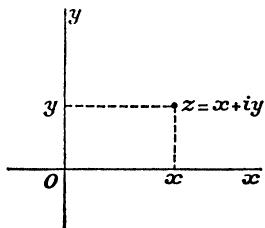
\includegraphics[keepaspectratio]{images/part001_cf49e1ad.jpg}}\\
图 7。

置换 \(z' \to \overline{z}\) （\(\mathbf{C}\) 的）是连续的，因此它是拓扑域 \(\mathbf{C}\) 的一个自同构。

事实上，它是拓扑域 C 中除恒等自同构外唯一的自同构（见习题 4）。

函数 \(\mathcal{R}(z)\) 、\(\mathfrak{J}(z)\) 正是 \(\mathbf{R}^2\) 到它的各因子上的投影，因此是连续的；绝对值 \(|z|\) 亦然，因为它是点 \((x,y)\) （在 \(\mathbf{R}^2\) 中）的欧氏范数（第六章，§ 2，第 1 号）。

绝对值的性质给出了 \(\mathbf{C}\) 的拓扑与其域结构相容这一事实的另一个证明（参看第九章，§ 3，第 2 号）；\(z + z'\) 的连续性由三角不等式 \(|z + z'| \leqslant |z| + |z'|\) 得出；\(zz'\) 的连续性由关系式

\[
\begin{array}{r l} | z z ^ {\prime} - z _ {0} z _ {0} ^ {\prime} | & = | z _ {0} (z ^ {\prime} - z _ {0} ^ {\prime}) + (z - z _ {0}) z _ {0} ^ {\prime} + (z - z _ {0}) (z ^ {\prime} - z _ {0} ^ {\prime}) | \\ & \leqslant | z _ {0} | \cdot | z ^ {\prime} - z _ {0} ^ {\prime} | + | z _ {0} ^ {\prime} | \cdot | z - z _ {0} | + | z - z _ {0} | \cdot | z ^ {\prime} - z _ {0} ^ {\prime} |; \end{array}
\]

得出；最后，\(z^{-1}\) 的连续性由关系式

\[
\left| z _ {0} ^ {- 1} - z ^ {- 1} \right| = | z | ^ {- 1}. \left| z - z _ {0} \right|. \left| z _ {0} \right| ^ {- 1}.
\]

\subsection{乘法群 C*}

我们从第三章 § 6 第 7 号知道，在非零复数的乘法群 \(\mathbf{C}^*\) 上诱导的拓扑与 \(\mathbf{C}^*\) 的群结构相容。由于 \(\mathbf{C}^*\) 在 \(\mathbf{C}\) 中是开的，由此得出 \(\mathbf{C}^*\) 是一个局部紧拓扑群（第一章，§ 9，第 7 号，命题 13），因而（关于乘法一致结构）是完备的；参看第三章，§ 6，第 8 号，命题 8）。乘法群 \(\mathbf{R}_+^*\) （\(>0\) 实数的）是 \(\mathbf{C}^*\) 的一个闭子群。另一个子群是绝对值为 1 的复数所成的集 \(\mathbf{U}\) ，它与单位圆周 \(\mathbf{S}_1\) （\(\mathbf{R}^2\) 的）等同，因此是一个紧群。此外：

命题 1. 拓扑群 \(\mathbf{C}^*\) 同构于拓扑群 \(\mathbf{R}^*\) 与 \(\mathbf{U}\) 的乘积。

因为映射 \(z \to \left( |z|, \frac{z}{|z|} \right)\) 是 \(\mathbf{C}^*\) 到 \(\mathbf{R}_+^* \times \mathbf{U}\) 上的一个同胚（第六章，§ 2，第 3 号，命题 3）；并且由此立即得出它是群结构的一个同构。

已经知道拓扑群 \(\mathbf{R}_{+}^{*}\) 同构于加法群 \(\mathbf{R}\) （第五章，§ 4，定理 1）；因此对拓扑群 \(\mathbf{C}^{*}\) 的研究就归结为对 \(\mathbf{U}\) 的研究，我们将在 § 2 中考虑它。

\subsection{四元数体}

由定理 1 推出，域 R 是一个极大有序域，因而（在同构意义下）R 上有限秩的唯一非交换除环就是 R 上的四元数体；它记作 H，称为实四元数体（或在无混淆之虞时简称四元数体）。由于 H 在域 R 上的秩为 4，我们可以在 H 上定义一个与 \(R^{4}\) 的拓扑同胚的拓扑（第六章，§ 1，第 5 号）。确切地说，我们通常把 H 与 \(R^{4}\) 等同，即把 H 的标准基的元素 1、i、j、k 分别等同于向量 \(e_{0}, e_{1}, e_{2}, e_{3}\) （\(R^{4}\) 的标准基的向量）。

我们回顾，H 的标准基的乘法表由下列公式给出

\[
\begin{array}{c} i ^ {2} = j ^ {2} = k ^ {2} = - \mathrm{I}, \quad i j = - j i = k, \\ j k = - k j = i, \quad k i = - i k = j. \end{array}
\]

H 的拓扑不仅与 H 的环结构相容（第六章，§ 1，第 5 号），而且与它的除环结构相容；因为若 x 是一个非零四元数，则 \(x^{-1}\) 的坐标是 x 的坐标的有理函数，其分母不为零。因此，赋有这一拓扑的除环 H 是一个非交换的拓扑除环。四元数 \(a + bi\) （a、b 为实数）构成 H 的一个（拓扑）子域，它同构于域 C，并常与 C 等同。

这样我们就有了局部紧、连通的拓扑除环的第三个例子，其余两个是 R 与 C。事实上，具有这两条性质的拓扑除环仅此三个。

我们从代数知道，四元数 \(x = x_{0} + x_{1}i + x_{2}j + x_{3}k\) 的约化范数是

\[
\mathrm{N} (\boldsymbol {x}) = x _ {0} ^ {2} + x _ {1} ^ {2} + x _ {2} ^ {2} + x _ {3} ^ {2} = | | \boldsymbol {x} | | ^ {2}
\]

（因此它是 x 的欧氏范数的平方）。由于

\[
\mathrm{N} (\boldsymbol {x y}) = \mathrm{N} (\boldsymbol {x}) \mathrm{N} (\boldsymbol {y}),
\]

由此得出，范数为 1 的所有四元数所成的集——它与球面 \(S_{3}\) 相同——构成非零四元数的乘法群 \(H^{*}\) 的一个紧子群。

命题 2. 非零四元数的乘法群 \(\mathbf{H}^*\) 是一个拓扑群，同构于它的子群 \(\mathbf{R}_+^*\) 与 \(\mathbf{S}_3\) 的乘积。

每个四元数 \(x \neq 0\) 都可以写成 \(x = ||x||.z\) ，其中 \(z\) 是范数为 1 的四元数；由于 \(||xx'|| = ||x||.||x'||\) ，映射 \(x \to (||x||, x/||x||)\) （\(H^*\) 到 \(R_+^* \times S_3\) 上的）是群结构的一个同构，并且由第六章 § 2 第 3 号命题 3，它是 \(H^*\) 到 \(R_+^* \times S_3\) 上的一个同胚。

注。1) 利用关系式 \(||x + y|| \leqslant ||x|| + ||y||\) 与 \(||xy|| = ||x||.||y||\) ，可以像第 2 号中对复数域那样直接证明 \(\mathbf{R}^4\) 的拓扑与 H 的除环结构相容（参看第九章，§ 3，第 2 号）。

\begin{enumerate}
\def\labelenumi{\arabic{enumi})}
\setcounter{enumi}{1}
\item
  由已证的结果推出，球面 \(S_{1}\) 与 \(S_{3}\) 能够带有与它们的拓扑相容的群结构。我们后面将看到，对每个异于 1 和 3 的整数 n，\(S_{n}\) 上不存在与 \(S_{n}\) 的拓扑相容的群结构。
\item
  群 \(\mathbf{S}_3\) 的每个点都有一个同胚于 \(\mathbf{R}^3\) 的邻域（第六章，§ 2，第 4 号，命题 5），但 \(\mathbf{S}_3\) 不局部同构于 \(\mathbf{R}^3\) ；因为若是这样，则由于它是连通的（第七章，§ 2，第 2 号，定理 1），它将是交换的，而事实并非如此，因为 \(i\) 与 \(j\) 都属于 \(\mathbf{S}_3\) 且 \(ij \neq ji\) （参看第五章，§ 3）。
\end{enumerate}

\section{角的测度，三角函数}

\subsection{乘法群 U}

定理 1. 绝对值为 1 的复数的（乘法）拓扑群 U 同构于模 1 实数的（加法）拓扑群 T。

\(\mathbf{U} = \mathbf{S}_{1}\) 是紧且连通的，并且它的单位元 \(+1\) 有一个同胚于 \(\mathbf{R}\) 的开区间的邻域（第六章，§ 2，第 4 号，命题 5）；因此该定理是第五章 § 3（定理 2）所给的 \(\mathbf{T}\) 的拓扑刻画的一个推论。

推论. 非零复数的乘法群 \(\mathbf{C}^*\) 同构于群 \(\mathbf{R} \times \mathbf{T}\) （参看 § 1. 第 3 号，命题 1）。

注. 群 \(C^{*}\) 与 \(R \times T\) 的同构蕴含着在域 C 中每个“二项方程” \(z^{n} = a\) 都有根。利用这一事实以及 C 的局部紧性，我们可以得到达朗贝尔–高斯定理的另一个证明（习题 2）。

从群 \(\mathbf{T}\) 到群 \(\mathbf{U}\) 上的不同同构只有两个；因为若 \(g\) 、\(g'\) 是 \(\mathbf{T}\) 到 \(\mathbf{U}\) 上的两个同构，而 \(h'\) 是 \(g'\) 的逆，则 \(h' \circ g\) 是 \(\mathbf{T}\) 的一个自同构，因而（第七章，§ 2，第 4 号，命题 6）我们恒有 \(g'(x) = g(x)\) 或 \(g'(x) = g(-x)\) 。我们总可以假设 \(g\) 使得 \(i\) 是 \(g\) 对模 \(1\) 类（点 \(\frac{1}{4}\) 的）所取的像；于是，若 \(\varphi\) 表示 \(\mathbf{R}\) 到 \(\mathbf{T}\) 上的典范同态，则加法群 \(\mathbf{R}\) 到乘法群 \(\mathbf{U}\) 上的每个严格态射都形如 \(x \to g(\varphi(x/a))\) ，其中 \(a\) 是一个 \(\neq o\) 的实数（第七章，§ 2，第 3 号，命题 4）；注意，区间 \([- \frac{1}{2} |a|, \frac{1}{2} |a|]\) 是 \(\mathbf{R}\) 中被这个严格态射一一地映到其像上的最大对称开区间，并且我们有 \(g(\varphi(\frac{1}{4})) = i\) 。我们将把同态 \(x \to g(\varphi(x))\) 记作 \(x \to e(x)\) ；因而 \(\mathbf{R}\) 到 \(\mathbf{U}\) 上的每个严格态射都形如 \(x \to e(x/a)\) ，其中 \(a \neq 0\) 。函数 \(e(x)\) 在 \(\mathbf{R}\) 上连续、取复值，并且满足恒等式

\begin{enumerate}
\def\labelenumi{(\arabic{enumi})}
\tightlist
\item
\end{enumerate}

\[
\left| e (x) \right| = 1,\tag{2}
\]

\[
\boldsymbol {e} (x + y) = \boldsymbol {e} (x) \boldsymbol {e} (y),
\]

以及关系式

\[
e (0) = \mathrm{I}, \quad e (\frac {1}{4}) = i, \quad e (\frac {1}{2}) = - \mathrm{I}, \quad e (\frac {3}{4}) = - i, \quad e (\mathrm{I}) = \mathrm{I}. \tag {3}
\]

由 (1) 与 (2) 得出

\[
e (- x) = \frac {1}{e (x)} = \overline {{{{e (x)}}}},\tag{4}
\]

而由 (2) 与 (3) 得出

\[
\begin{array}{l} e (x + \frac {1}{4}) = i e (x), \quad e (x + \frac {1}{2}) = - e (x), \\ e (x + \frac {3}{4}) = - i e (x), \quad e (x + 1) = e (x). \end{array}
\]

于是函数 \(e(x)\) 是周期的，并且以 1 为基本周期。

注. 映射 \(x + iy \to e^x e(y)\) 是加法群 \(\mathbf{C}\) 到乘法群 \(\mathbf{C}^*\) 上的一个严格态射，并且它在 \(\mathbf{o}\) 的一个适当邻域上的限制是 \(\mathbf{C}\) 与 \(\mathbf{C}^*\) 的一个局部同构。因而（第七章，§ 2，第 3 号）\(\mathbf{C}\) 到 \(\mathbf{C}^*\) 上的每个严格态射都形如 \(x + iy \to e^{\alpha x + \beta y} e(\gamma x + \delta y)\) ，其中 \(\alpha, \beta, \gamma, \delta\) 是使 \(\alpha \delta - \beta \gamma \neq \mathbf{o}\) 的任意实数。我们后面将看到，这些同态中恰有一个，记作 \(z \rightarrow e^{z}\) ，使得

\[
\lim _ {z \rightarrow 0} \frac {e ^ {z} - 1}{z} = 1;
\]

并且这个同态在实轴上的限制与 \(e^{x}\) 相同（由此得到该记号）。

\subsection{角}

由于域 \(\mathbf{R}\) 是有序的，我们可以定向实数平面 \(\mathbf{R}^2\) ，方法是取 \(e_1 \wedge e_2\) 为正二重向量（\(e_1, e_2\) 是标准基的向量）。于是，在定向的实数平面 \(\mathbf{R}^2\) （以下与 \(\mathbf{C}\) 等同）中，我们可以对任意一对射线定义角 \((\widehat{\Delta_1, \Delta_2})\) （射线对（ \(\Delta_1, \Delta_2\) ）以 \(o\) 为端点）(*)。所有角组成的集合 \(\mathfrak{A}\) 具有一个交换群结构（写成加法），由下式定义

\[
(\widehat {\Delta_ {1} , \Delta_ {3}}) = (\widehat {\Delta_ {1} , \Delta_ {2}}) + (\widehat {\Delta_ {2} , \Delta_ {3}}),
\]

于是特别有 \((\widehat{\Delta_1, \Delta_1}) = 0\) 且 \((\widehat{\Delta_2, \Delta_1}) = -(\widehat{\Delta_1, \Delta_2})\) 。

平角 \(\varpi\) 是 \(\neq 0\) 的解，即方程 \(2\theta = 0\) 在 \(\mathfrak{A}\) 中的解；它是负实半轴与正实半轴所成的角。

若 z 是任一非零复数，z 的辐角（或幅角），记作 \(\operatorname{Am}(z)\) ，是过 z 而以 o 为端点的射线与正实半轴所成的角。映射 \(z \to \operatorname{Am}(z)\) 是乘法群 \(C^{*}\) 到加法群 A 上的一个同态，因而我们有

\[
\operatorname{Am} \left(z z ^ {\prime}\right) = \operatorname{Am} (z) + \operatorname{Am} \left(z ^ {\prime}\right) \quad \text { and } \quad \operatorname{Am} (\bar {z}) = \operatorname{Am} \left(z ^ {- 1}\right) = - \operatorname{Am} (z).
\]

角 \(\delta = \operatorname{Am}(i)\) 称为正直角；它是方程 \(2\theta = \varpi\) 在 A 中的解之一，另一个解是 \(-\delta = \delta + \varpi\) 。

同态 \(z \to \operatorname{Am}(z)\) 限制到子群 \(\mathbf{U}\) （\(\mathbf{C}^*\) 的）上时，是 \(\mathbf{U}\) 的群结构到 \(\mathfrak{A}^{(**)}\) 的群结构上的一个同构；若用这个同构把 U 的拓扑转移到群 A 上，则后一群成为一个紧拓扑群，并且映射 \(z \to \operatorname{Am}(z)\) （\(C^{*}\) 到 A 上的）是拓扑群 \(C^{*}\) 到拓扑群 A 上的一个严格态射。

我们把 \(\theta \to f(\theta)\) 记为 \(\mathfrak{A}\) 到 \(\mathbf{U}\) 上的同构，它即同构 \(z \to \operatorname{Am}(z)\) （\(\mathbf{U}\) 到 \(\mathfrak{A}\) 上的）的逆。按定义，\(\mathcal{R}(f(\theta))\) 记作 \(\cos \theta\) ，称为角 \(\theta\) 的余弦；\(\mathfrak{J}(f(\theta))\) 记作 \(\sin \theta\) ，称为角 \(\theta\) 的正弦。这些函数在拓扑群 \(\mathfrak{A}\) 上连续，并且满足下列关系式（同处所引），它们是上述定义的直接推论：

\[
\begin{array}{r l} \cos o = 1, & \sin o = 0, \quad \cos \varpi = - 1, \quad \sin \varpi = 0, \\ \cos (- \theta) = \cos \theta , & \sin (- \theta) = - \sin \theta , \\ \cos (\theta + \theta^ {\prime}) = \cos \theta \cos \theta^ {\prime} - \sin \theta \sin \theta^ {\prime}, \\ \sin (\theta + \theta^ {\prime}) = \sin \theta \cos \theta^ {\prime} + \sin \theta^ {\prime} \cos \theta , \\ \cos^ {2} \theta + \sin^ {2} \theta = 1. \end{array}
\]

按定义，角 \(\theta \in \mathfrak{A}\) 的正切，当 \(\cos \theta \neq 0\) 时定义为 \(\sin \theta / \cos \theta\) （同处所引），记作 \(\tan \theta\) ；它是一个连续函数，由连续性延拓到 \(\tilde{\mathbf{R}}\) （第六章，§ 3，第 4 号），即取值 \(\infty\) 于角 \(\delta\) 与 \(-\delta\) 处。我们有 \(\tan (\theta + \varpi) = \tan \theta\) 。\(\theta\) 的余切，记作 \(\cot \theta\) ，是 \(\tilde{\mathbf{R}}\) 中等于 \(1 / \tan \theta\) 的元素。

注意，若 \(\operatorname{Am}(z) = \theta\) ，我们有 \(z = |z| (\cos \theta + i \sin \theta)\) ；这个表达式称为复数 \(z \neq 0\) 的三角形式。

\subsection{角的测度}

由第 1 号的定理 1，角的拓扑群 \(\mathfrak{A}\) 同构于 \(\mathbf{T}\) 。\(\mathbf{R}\) 到 \(\mathfrak{A}\) 上的每个严格态射都可由同构 \(z \to \operatorname{Am}(z)\) （\(\mathbf{U}\) 到 \(\mathfrak{A}\) 上的）与 \(\mathbf{R}\) 到 \(\mathbf{U}\) 上的一个严格态射复合而得；若令 \(\Im(x) = \operatorname{Am}(e(x))\) ，则 \(\mathbf{R}\) 到 \(\mathfrak{A}\) 上的每个严格态射都形如 \(x \to \Im(x/a)\) （ \(a \neq 0\) ）。给定一个一劳永逸地固定的实数 \(a > 0\) ，每个角 \(\theta\) 经同态 \(x \to \Im(x/a)\) 对应于实数模 \(a\) 的一个类（即 \(\mathbf{Z}/a\mathbf{Z}\) 的一个元素），它称为 \(\theta\) 相对于底 \(a\) 的测度；按惯用说法，该类中的每个实数也称为 \(\theta\) 的一个测度；角 \(\Im(x/a)\) 称为（相对于底 a）测度为 \(x\) 的角。若 x 是 \(\theta\) 的一个测度而 \(x'\) 是 \(\theta'\) 的一个测度（相对于同一个底），则 \(x + x'\) 是 \(\theta + \theta'\) 的一个测度，且 -x 是 - \(\theta\) 的一个测度。角（相对于底 a）的主测度是其位于区间 {[}0, a{]} 中的那个测度。

底 \(a\) 的选取。我们总限于取 \(a > 1\) 的底。每个 \(a > 1\) 对应一个角 \(\omega = \Im(1/a)\) ，它的主测度是 \(1\) ，称为相对于底 \(a\) 的角的测度单位；反之，每个角 \(\omega \neq 0\) 对应唯一的 \(a > 1\) 使 \(\Im(1/a) = \omega\) ，因此知道角的测度单位就完全确定了底 \(a > 1\) 。

在数值计算中通常取 \(a = 360\) 或 \(a = 400\) ；相应的角的测度单位称为度（ \(a = 360\) ）或百分度（ \(a = 400\) ）。

在分析中，以及在一切不涉及数值计算的数学分支中，普遍使用由条件

\[
\lim _ {x \rightarrow 0} \frac {e (x / a) - 1}{x} = 1
\]

所定义的底 a；这个底记作 \(2\pi\) 。相应的角的测度单位称为弧度，其测度称为弧度测度；利用前面提到的对复数 z 的 \(e^{z}\) 的定义，我们有 \(\boldsymbol{e}(x)=e^{2\pi ix}\) 对一切 \(x\in R\) 成立。

底 a 一经选定，当人们说到一个角时，通常指的就是这个角相对于底 a 的一个测度；只要（在不涉及数值计算时情形总是如此）底 a 自始至终保持固定，并且记住模 a 同余的两个实数对应于同一个角，这种惯用说法并无妨碍。

例如，通常所理解的复数 \(z \neq 0\) 的辐角，是指该角的一个弧度测度，它由依所考虑的问题而定的约定来确定；这些约定一经作出，如此选定的辐角的测度就记作 Am (z)。

\subsection{三角函数}

若把（定义在 A 上的）函数 \(\cos\theta\) 、\(\sin\theta\) 、\(\tan\theta\) 、\(\cot\theta\) 与 R 到 A 上的同态 \(x\to\Im(x/a)\) 复合，则如此得到的函数

\[
\cos \Im \left(\frac {x}{a}\right), \quad \sin \Im \left(\frac {x}{a}\right), \quad \tan \Im \left(\frac {x}{a}\right), \quad \cot \Im \left(\frac {x}{a}\right)
\]

分别称为数 \(x\) 相对于底 \(a\) 的余弦、正弦、正切与余切，并记作 \(\cos_a x\) 、\(\sin_a x\) 、\(\tan_a x\) 、\(\cot_a x\) 。映射 \(x \to \cos_a x + i \sin_a x\) 是 \(\theta \to \cos \theta + i \sin \theta\) 与 \(x \to \Im(x/a)\) 的复合，因而由第 2 号中 \(\cos \theta\) 与 \(\sin \theta\) 的定义，我们有恒等式

\[
e \left(\frac {x}{a}\right) = \cos_ {a} x + i \sin_ {a} x,\tag{5}
\]

它等价于

\[
\cos_ {a} x = \Re \left(e \left(\frac {x}{a}\right)\right), \quad \sin_ {a} x = \Im \left(e \left(\frac {x}{a}\right)\right),
\]

并且由 (4)，它也等价于

\[
\cos_ {a} x = \frac {\mathrm{I}}{2} \left(e \left(\frac {x}{a}\right) + e \left(- \frac {x}{a}\right)\right), \quad \sin_ {a} x = \frac {\mathrm{I}}{2 i} \left(e \left(\frac {x}{a}\right) - e \left(- \frac {x}{a}\right)\right).
\]

由此得到恒等式

\[
\cos_ {b} x = \cos_ {a} \left(\frac {a x}{b}\right), \quad \sin_ {b} x = \sin_ {a} \left(\frac {a x}{b}\right).\tag{6}
\]

在不涉及数值计算的数学分支中所出现的三角函数，只有上述相对于基 \(2\pi\) 的那些函数；这些函数简单地记作 \(\cos x\) 、\(\sin x\) 、\(\tan x\) 、\(\cot x\) ，以代替 \(\cos_{2\pi}x\) 、\(\sin_{2\pi}x\) 、\(\tan_{2\pi}x\) 、\(\cot_{2\pi}x\) 。出于数值计算的目的，有对应于基 a = 360 与 a = 400 的三角函数表；而公式 (6) 使我们能推出相对于任何其他基的三角函数的值。

前面回忆过的角的余弦与正弦之间的关系，显然给出度量这些角的数之间的同样的关系；特别地，我们有

\[
\begin{array}{r l} & {\cos_ {a} (x + y) = \cos_ {a} x \cos_ {a} y - \sin_ {a} x \sin_ {a} y,} \\ & {\sin_ {a} (x + y) = \sin_ {a} x \cos_ {a} y + \sin_ {a} y \cos_ {a} x,} \\ & {\cos_ {a} (- x) = \cos_ {a} x, \qquad \sin_ {a} (- x) = - \sin_ {a} x,} \\ & {\qquad \cos_ {a} ^ {2} x + \sin_ {a} ^ {2} x = 1.} \end{array}
\]

函数 \(\cos_{a}x\) 与 \(\sin_{a}x\) 在 R 上连续，并且以 a 为周期；此外，a 是这些函数的基本周期，因为关系 \(\cos_{a}x = \cos_{a}y\) 蕴含或者 \(\sin_{a}x = \sin_{a}y\) ，或者

\[
\sin_ {a} x = - \sin_ {a} y, \quad \text { i.e., }
\]

\[
e \left(\frac {x}{a}\right) = e \left(\frac {y}{a}\right) \quad \text { or } \quad e \left(\frac {x}{a}\right) = e \left(- \frac {y}{a}\right),
\]

从而或者

\[
x \equiv y (\mathrm{mod} a) \quad \text { or } \quad x \equiv - y (\mathrm{mod} a);
\]

而类似地，

\[
\sin_ {a} x = \sin_ {a} y
\]

等价于 \(x \equiv y \pmod{a}\) 或者 \(x + y \equiv \frac{1}{2} a \pmod{a}\) 。

由此可知，\(\cos_{a}x\) 在区间 \([0,\frac{1}{2}a]\) 中绝不两次取同一个值；因此，当限制在这个区间上时，它是该区间到区间 \([-1,+1]\) 上的一个双射映射。由于 \(\cos_{a}0=1\) 且 \(\cos_{a}\left(\frac{1}{2}a\right)=-1\) ，故 \(x\to\cos_{a}x\) 是 \([0,\frac{1}{2}a]\) 到 \([-1,1]\) 上的一个严格递减映射（第四章，§ 2，第 6 号，定理 5 及其注）。\(\cos_{a}x=0\) （当 x=a/4），\(\cos_{a}x>0\) 对 \(0\leqslant x<a/4\) 成立，\(\cos_{a}x<0\) 对 \(a/4<x\leqslant a/2\) 成立。由 \(\cos_{a}(-x)=\cos_{a}x\) 可以推出 \(\cos_{a}x\) 在区间 \([-\frac{1}{2}a,0]\) 中的变化情况，从而由周期性推出它在整个 R 上的变化情况（图 8）。由 \(\sin_{a}x=-\cos_{a}(x+a/4)\) 又可推出 \(\sin_{a}x\) 在 R 中的变化情况（图 8）。

\pandocbounded{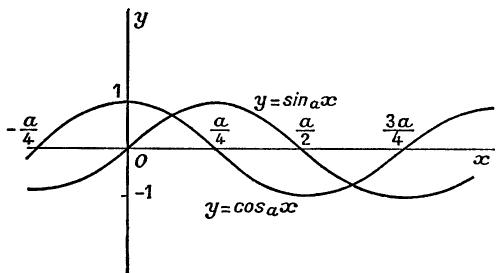
\includegraphics[keepaspectratio]{images/part001_7529c0a8.jpg}}\\
图 8.

函数 \(\tan_{a}x\) 是 \(\mathbf{R}\) 到 \(\tilde{\mathbf{R}}\) 上的一个连续映射；它取值 \(\infty\) 于诸值 \(\frac{1}{4} a + \frac{1}{2} ka\) 处（ \(k \in \mathbf{Z}\) ）。由于 \(\frac{1}{2} a\) 是 \(\tan_{a}x\) 的一个周期，故它是一个基本周期。在区间 \([0, \frac{1}{4} a]\) 中，\(\sin_{a}x\) 从 \(0\) 递增到 \(1\) ，\(\cos_{a}x\) 从 \(1\) 递减到 \(0\) ，因此 \(\tan_{a}x\) 在 \([0, \frac{1}{4} a[\) 中严格递增，并把这个区间映射到 \([0, +\infty[\) 上；由此推出 \(\tan_{a}x\) 在区间 \(]-\frac{1}{4}a,+\frac{1}{4}a[.\) 中严格递增，并且是这个区间到 R 上的一个同胚（图 9）。

\pandocbounded{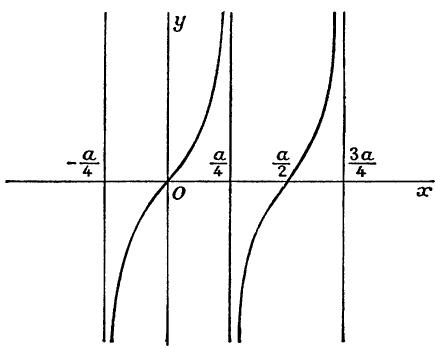
\includegraphics[keepaspectratio]{images/part001_329f289a.jpg}}\\
图 9.

\subsection{角域}

给定两条不同的闭射线 \(\Delta_{1}, \Delta_{2}\) ，其端点为 \(o\) ，设 \(x\) 为角 \((\widehat{\Delta_{1}, \Delta_{2}})\) 的主测度（相对于一个基 \(a\) ，一经选定便不再改变）。闭（相应地开）射线 \(\Delta\) （以 \(o\) 为端点）当中，其主测度 \(y\) （角 \((\widehat{\Delta_{1}, \Delta})\) 的）满足 \(o \leqslant y \leqslant x\) （相应地 \(o < y < x\) ）者的并集，就是代数中所定义的闭（相应地开）角域 \(S\) （以 \(\Delta_{1}\) 为始边、以 \(\Delta_{2}\) 为终边）。因为借助于一个旋转，总可以化归为 \(S\) 不包含过点 \(-1\) 的射线的情形。若 \(\alpha\) 与 \(\beta\) 此时是 \(\Delta_{1}\) 与 \(\Delta_{2}\) 分别与实正半轴所成的角，则闭角域 \(S\) 是诸闭半直线 \(\Delta\) 的并，这些半直线与实正半轴成角 \(\theta\) ，使得 \(\tan \frac{1}{2} \alpha \leqslant \tan \frac{1}{2} \theta \leqslant \tan \frac{1}{2} \beta\) 。而若 \(u, v, t\) 分别是 \(\alpha, \beta, \theta\) 的属于区间 \([- \frac{1}{2} a, + \frac{1}{2} a[\) 的测度，则这些不等式等价于 \(\tan_{a} \frac{1}{2} u \leqslant \tan_{a} \frac{1}{2} t \leqslant \tan_{a} \frac{1}{2} v\) ；又由于 \(\tan_{a} x\) 在区间 \([- \frac{1}{4} a, + \frac{1}{4} a[\) 中是递增函数，它们也等价于 \(u \leqslant t \leqslant v\) ，或等价于 \(o \leqslant t - u \leqslant v - u\) ；由于 \(x = v - u\) ，\(y = t - u\) ，于是结论对闭角域得证，而对开角域的证明是类似的。

闭角域是 \(R^{2}\) 中的闭集，而与它有同一始边和同一终边的开角域是它在 \(R^{2}\) 中的内部（第六章，§ 2，第 3 号，命题 3）。角 \((\widehat{\Delta_1, \Delta_2})\) （其主测度为 \(x\) ）称为角域 S 的角；当 \(x < \frac{1}{2} a\) 时称 S 为凸角域，当 \(x = \frac{1}{2} a\) 时称为平角域（即闭半平面），当 \(x > \frac{1}{2} a\) 时称为凹角域。凸角域当 \(x < \frac{1}{4} a\) 时为锐角域，当 \(x = \frac{1}{4} a\) 时为直角域，当 \(x > \frac{1}{4} a\) 时为钝角域。角域 S 的平分线是射线 \(\Delta\) ，它以 \(y = \frac{1}{2} x\) 为其与 \(\Delta_1\) 所成的角。

\pandocbounded{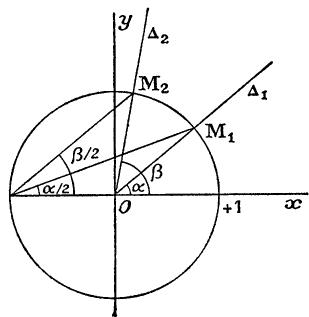
\includegraphics[keepaspectratio]{images/part001_1c4c55ab.jpg}}\\
图 10.

两条不同的闭射线 \(\Delta_{1}, \Delta_{2}\) 确定两个闭角域；它们的并是实平面 \(R^{2}\) ，而它们的交是 \(\Delta_{1} \cup \Delta_{2}\) 。

\subsection{叉角}

我们也在代数中定义过极大有序域上的二维向量空间中一对直线的叉角（*）。这个定义特别适用于实平面 \(\mathbf{R}^2\) 。全体叉角的集合 \(\mathfrak{A}_0\) 具有一个交换群结构（写成加法），它由下式定义

\[
(\widehat {\mathbf {D _ {1} , D _ {3}}}) = (\widehat {\mathbf {D _ {1} , D _ {2}}}) + (\widehat {\mathbf {D _ {2} , D _ {3}}})
\]

因而特别有 \((\widehat{\mathbf{D}_1,\mathbf{D}_1}) = 0\) 与 \((\widehat{\mathbf{D}_2,\mathbf{D}_1}) = -(\widehat{\mathbf{D}_1,\mathbf{D}_2}).\)

直叉角 \(\delta_0\) 是 \(\neq 0\) 的、方程 \(2\theta = 0\) 在 \(\mathfrak{A}_0\) 中的解；它是虚轴与实轴所成的叉角。

我们定义一个典范同态 \(\varphi\) ：由角群 \(\mathfrak{A}\) 到叉角群 \(\mathfrak{A}_0\) 上，它把射线 \(\Delta\) 与实正半轴所成的角，对应为包含 \(\Delta\) 的直线 D 与实轴所成的叉角。一个叉角 \(\theta_0\) 是 \(\varphi\) 下两个角 \(\theta\) 与 \(\theta + \varpi\) 的像；于是 \(\mathfrak{A}_0\) 同构于 \(\mathfrak{A}\) 对子群 \(\{o, \varpi\}\) 的商群。若在 \(\mathfrak{A}_0\) 上转移商群 \(\mathfrak{A}/\{o, \varpi\}\) 的拓扑（借助与 \(\varphi\) 相伴的双射同态来转移），则 \(\mathfrak{A}_0\) 成为一个紧拓扑群，而 \(\varphi\) 成为 \(\mathfrak{A}\) 到 \(\mathfrak{A}_0\) 上的一个严格态射。

如果把同态 \(\varphi\) （ \(\mathfrak{A}\) 到 \(\mathfrak{A}_0\) 上的）与同态 \(x \to \Im(x/a)\) （ \(\mathbf{R}\) 到 \(\mathfrak{A}\) 上的）复合，就得到一个同态 \(x \to \Im_0(x/a)\) （ \(\mathbf{R}\) 到 \(\mathfrak{A}_0\) 上的）；每个叉角 \(\theta_0 \in \mathfrak{A}_0\) 在这个同态之下对应于实数的一个模 \(\frac{1}{2}a\) 的类，它称为叉角 \(\theta_0\) 的测度（相对于基 \(a\) ）；照惯用说法，这个类中的每个数都称为 \(\theta_0\) 的一个测度，而其中属于区间 \([0, \frac{1}{2}a]\) 的那个称为 \(\theta_0\) 的主测度；叉角 \(\Im_0(x/a)\) 是测度为 \(x\) 的叉角。\(\theta_0\) 的每个测度也是角 \(\theta, \theta + \varpi\) 二者之一的一个测度，这两个角在同态 \(\varphi\) 下的像是 \(\theta_0\) 。

这里同样地，一旦选定了基 a ，当我们谈到一个叉角时，照惯用说法，一般指相对于基 a 的这个叉角的一个测度。

注。我们可以定义 \(\mathbf{C}^*\) 到 \(\mathfrak{A}_0\) 上的一个同态，它把每个复数 \(z \neq 0\) 映为过 \(0\) 与 \(z\) 的直线与实轴所成的叉角。显然这个同态是 \(\varphi\) 与同态 \(z \to \operatorname{Am}(z)\) （ \(\mathbf{C}^*\) 到 \(\mathfrak{A}\) 上的）的复合；因此它是拓扑群 \(\mathbf{C}^*\) 到拓扑群 \(\mathfrak{A}_0\) 上的一个严格态射，而与之相伴的双射同态是商群 \(\mathbf{C}^*/\mathbf{R}^*\) 到 \(\mathfrak{A}_0\) 上的一个同构。

我们知道，若 D 表示一条与实轴成叉角 \(\theta_0\) 的直线，且 \((a, b)\) 是 D 的一对方向比，则叉角 \(\theta_0\) 的正切（记作 tan \(\theta_0\) ）是元素 \(b/a\) （ \(\tilde{\mathbf{R}} (= \infty\) 若 \(a = 0\) ），它也称为直线 D 的斜率。若 \(\theta\) 与 \(\theta + \varpi\) 是在 \(\varphi\) 下以 \(\theta_0\) 为像的两个角，则有 \(\tan \theta_0 = \tan \theta = \tan (\theta + \varpi)\) 。映射 \(\theta_0 \to \tan \theta_0\) 是 \(\mathfrak{A}_0\) 到 \(\tilde{\mathbf{R}}\) 上的一个同胚，因为拓扑空间 \(\mathbf{C}^*/\mathbf{R}^*\) 正是实射影直线 \(\mathbf{P}_1\) ，而且由第六章 § 3 第 3 号，把直线（视为 \(\mathbf{P}_1\) 的点）对应到其斜率的映射是 \(\mathbf{P}_1\) 到 \(\tilde{\mathbf{R}}\) 上的一个同胚。现在，若在 \(\tilde{\mathbf{R}}\) 上转移 \(\mathfrak{A}_0\) 的群结构（借助映射 \(\theta_0 \to \tan \theta_0\) 来转移），我们就在 \(\tilde{\mathbf{R}}\) 上定义了一个交换拓扑群的结构，其中两个元素 \(t_1\) 、\(t_2\) 的积是 \(\frac{t_1 + t_2}{1 - t_1 t_2}\) ，只要 \(t_1\) 、\(t_2\) 属于 R 且 \(t_1 t_2 \neq 1\) ；对不满足这些条件的数对 \((t_1, t_2)\) ，\(t_{1}\) 与 \(t_{2}\) 的积通过把函数 \(\frac{x+y}{1-xy}\) 连续地延拓到 \(\tilde{R}\times\tilde{R}\) 而得到，并且仍记作 \(\frac{t_{1}+t_{2}}{1-t_{1}t_{2}}\) 。

\section{复数的无穷和与无穷乘积}

\subsection{复数的无穷和}

由于域 C 的加法群与加法群 \(R^{2}\) 相同，无须对 C 中的可和族与级数作专门研究，因为这已包含在第七章 § 3 的一般理论之中；我们把这理论的结果翻译成复数理论的语言这一练习留给读者。我们只叙述下面的命题，它是第七章 § 3 第 1 号命题 3 的一个推论：

命题 1 。若 \((u_{\lambda})_{\lambda \in \mathbf{L}}\) 与 \((v_{\mu})_{\mu \in \mathbf{M}}\) 是两个复数的可和族，则族 \((u_{\lambda}v_{\mu})_{(\lambda ,\mu)\in \mathbf{L}\times \mathbf{M}}\) 可和，且有

\[
\sum_ {(\lambda , \mu) \in \mathbf {L} \times \mathbf {M}} u _ {\lambda} v _ {\mu} = \left(\sum_ {\lambda \in \mathbf {L}} u _ {\lambda}\right) \left(\sum_ {\mu \in \mathbf {M}} v _ {\mu}\right).\tag{1}
\]

把关于四元数的相应结果的叙述留给读者。

\subsection{\texorpdfstring{\(C^*\) 中的可乘族}{复数乘法群中的可乘族}}

在非零复数的乘法群 \(\mathbf{C}^*\) 中，一个族 \((z_{i})_{i\in I}\) 只有当 \(\lim z_{i} = 1\) （关于 \(I\) 的有限子集的余集所成的滤子）时才可能是可乘的（第三章，§ 5，第 2 号，命题 1）；此外，由于 \(\mathbf{C}^*\) 的每一点都有可数的基本邻域系，指标 \(i\) （满足 \(z_{i}\neq 1\) 者）所成的集合当族 \((z_{i})\) 可乘时是可数的（第三章，§ 5，第 2 号，命题 1 的推论）。

命题 2 。复数的一个族 \((z_{t})\) ，其中 \(z_{t} = r_{t}(\cos \theta_{t} + i\sin \theta_{t})\) ，它是可乘的，当且仅当族 \((r_{t})\) （诸 \(z_{t}\) 的绝对值所成的）在 \(\mathbf{R}_{+}^{*}\) 中可乘，且族 \((\theta_{t})\) （诸 \(z_{t}\) 的辐角所成的）在角群 \(\mathfrak{A}\) 中可和。

鉴于群 \(\mathbf{C}^*\) 的结构（ \(\S\) 1，第 3 号，命题 1），本命题是第三章 \(\S\) 5 第 4 号命题 4 的直接推论。

若把每个角 \(\theta\) 映到它的（对任给基 \(a\) 而言的）属于区间 \([- \frac{1}{2} a, \frac{1}{2} a]\) 的那个测度，就得到 \(\mathfrak{A}\) 与 \(\mathbf{R}\) 的一个局部同构（ \(\S 2\) ，第 2 号）；由于 \(\lim \theta_{t} = 0\) （关于 \(\mathbf{I}\) 的有限子集的余集所成的滤子），我们可以把（命题 2 陈述中的）族 \(\theta_t\) 在 \(\mathfrak{A}\) 中可和这一条件，换成这样的条件：族 \((t_t)\) （诸角 \(\theta_t\) 的、属于 \([- \frac{1}{2} a, \frac{1}{2} a]\) 的测度所成之族）在 \(\mathbf{R}\) 中可和。

下述定理给出了形如 \((\mathbf{1} + u_{\iota})\) 的复数族在 \(\mathbf{C}^*\) 中可乘的另一个判别法。（它推广了第四章 § 7 第 4 号的定理 4；并参见第九章附录第 2 号命题 1：）

定理 1 。族 \((\mathbf{1} + u_{\iota})_{\iota \in \mathbf{I}}\) 在 \(\mathbf{C}^*\) 中可乘的充分必要条件是：族 \((|u_{\iota}|)\) 在 \(\mathbf{R}\) 中可和。

对 I 的每个有限子集 J，令

\[
p _ {J} = \prod_ {\iota \in J} (\mathbf{1} + a _ {\iota}), \quad s _ {J} = \sum_ {\iota \in J} a _ {\iota}, \quad \sigma_ {J} = \sum_ {\iota \in J} | a _ {\iota} |.
\]

引理 1 。对 I 的每个有限子集 J，令 \(\varphi(J) = \sup_{L \subset J} (p_L - 1)\) 。则对 J 的每个子集 L，我们有

\[
\left| p _ {\mathbf {L}} - \mathbf {1} - s _ {\mathbf {L}} \right| \leqslant \varphi (\mathrm{J}) \sigma_ {\mathbf {L}}.\tag{2}
\]

当 L 为空集时这是明显的。我们对 card (L) 作归纳。设 \(L = K \cup \{\lambda\}\) ，其中 \(\lambda \notin K\) ；则 \(p_{\mathbf{L}} = p_{\mathbf{K}}(\mathbf{1} + a_{\lambda})\) 且 \(s_{\mathbf{L}} = s_{\mathbf{K}} + a_{\lambda}\)，从而 \(p_{\mathbf{L}} - \mathbf{1} - s_{\mathbf{L}} = (p_{\mathbf{K}} - \mathbf{1} - s_{\mathbf{K}}) + (p_{\mathbf{K}} - \mathbf{1})a_{\lambda}\) ；于是由归纳假设与 \(\varphi(\mathbf{J})\) 的定义，有

\[
\left| p _ {\mathrm{L}} - \mathrm{1} - s _ {\mathrm{L}} \right| \leqslant \varphi (\mathrm{J}) \sigma_ {\mathrm{K}} + \varphi (\mathrm{J}) \left| a _ {\lambda} \right| = \varphi (\mathrm{J}) \sigma_ {\mathrm{L}},
\]

这就证明了引理。

引理 2 。若 J 是 I 的使 \(\varphi(J) < 1/4\) 的有限子集，则

\[
\left| \sigma_ {J} \right| \leqslant 4 \varphi (J) / (1 - 4 \varphi (J)).
\]

因为 \(\sigma_{\mathbf{L}} \leqslant \sigma_{\mathbf{J}}\) 对子集 \(\mathbf{L}\) （ \(\mathbf{J}\) 的每一个）成立，故由 (2) 得 \(|s_{\mathbf{L}}| \leqslant \varphi(\mathbf{J})\sigma_{\mathbf{J}} + |p_{\mathbf{L}} - \mathbf{1}| \leqslant (\mathbf{1} + \sigma_{\mathbf{J}})\varphi(\mathbf{J})\) ；但由第七章 §3 第 1 号命题 2，有 \(|\sigma_{\mathbf{J}}| \leqslant 4\sup_{\mathbf{L} \subset \mathbf{J}} |s_{\mathbf{L}}|\) ，从而 \(\sigma_{\mathbf{J}} \leqslant 4\varphi(\mathbf{J})(\mathbf{1} + \sigma_{\mathbf{J}})\) ，由此即得结论。

现在来证明定理 1 所述的条件是充分的。族 \((|u_{\iota}|)\) 在 \(\mathbf{R}\) 中可和这一假设蕴含族 \((\mathrm{1} + |u_{\iota}|)\) 在 \(\mathbf{R}_{+}^{*}\) 中可乘（第四章，§ 7，第 4 号，定理 4）；因此，对每个 \(\varepsilon > 0\) ，存在 I 的有限子集 \(J_{0}\) ，使得对每个不与 \(J_{0}\) 相交的 I 的有限子集 L，有 \(\prod_{\iota \in L} (\mathrm{1} + |u_{\iota}|) - \mathrm{1} \leqslant \varepsilon\) 。但我们可以把 \(\prod_{\iota \in L} (\mathrm{1} + u_{\iota}) - \mathrm{1}\) 写成 \(\sum_{M} \left( \prod_{\iota \in M} u_{\iota} \right)\) 的形式，其中 M 取遍 L 的所有非空子集；而由于 \(\left| \prod_{\iota \in M} u_{\iota} \right| = \prod_{\iota \in M} |u_{\iota}|\) ，我们有

\[
\left| \prod_ {\iota \in L} (1 + u _ {\iota}) - 1 \right| \leqslant \sum_ {M} \left(\prod_ {\iota \in M} | u _ {\iota} |\right) = \prod_ {\iota \in L} (1 + | u _ {\iota} |) - 1 \leqslant \varepsilon .
\]

由于 \(\mathbf{C}^*\) 是完备群，根据柯西判别法，这就证明了我们的断言。

还须证明定理 1 的条件是必要的。若 \((\mathbf{1} + u_{\iota})_{\iota\in \mathbf{I}}\) 是 \(\mathbf{C}^*\) 中的可乘族，则存在一个有限子集 \(J\) （ \(I\) 的），使得对每个有限子集 \(H\) （ \(I\) 的、不与 \(J\) 相交的），有 \(\left|\prod_{\iota\in H}(1 + u_{\iota}) - 1\right| \leqslant 1/8\) 。由引理 2 推出，\(\sum_{\iota\in H}|u_{\iota}| \leqslant 1\) 对每个有限子集 \(H\) （ \(I\) 的、不与 \(J\) 相交的）成立，因而族 \((|u_{\iota}|)\) 在 \(\mathbf{R}\) 中可和（第四章，§ 7，第 1 号，定理 1）。

上面的证明经过适当修改，也适用于某些非交换除环和代数中的（有序）无穷乘积（见习题 6 及第九章附录）。

\subsection{复数的无穷乘积}

为使以 \(z_{n} = r_{n}(\cos \theta_{n} + i\sin \theta_{n})\) 为通项的非零复数的无穷乘积在 \(\mathbf{C}^{*}\) 中收敛，根据群 \(\mathbf{C}^{*}\) 的结构，必要且充分的是：以 \(r_{n}\) 为通项的乘积在 \(\mathbf{R}_{+}^{*}\) 中收敛，且以 \(t_{n}\) 为通项的级数（即 \(\theta_{n}\) 的属于 \(] - \frac{1}{2} a, \frac{1}{2} a]\) 的测度）在 \(\mathbf{R}\) 中收敛。

定义 1 。以 \(1 + u_{n}\) 为通项的复数无穷乘积称为绝对收敛的，如果以 \(1 + |u_{n}|\) 为通项的乘积收敛（或者等价地，以 \(|u_{n}|\) 为通项的级数收敛）。

命题 3 。复数的无穷乘积交换收敛，当且仅当它绝对收敛。

这由第三章 § 5 第 7 号的命题 9 及上面第 2 号的定理 1 得出。

注。1) 以 \(|1 + u_n|\) 为通项的乘积可以在 \(\mathbf{R}_+^*\) 中收敛甚至绝对收敛，而以 \(1 + |u_n|\) 为通项的乘积不收敛（见习题 4）；当然，若诸 \(u_n\) 从某个下标起都是实数且 \(>0\) ，这种情形不会发生。

\begin{enumerate}
\def\labelenumi{\arabic{enumi})}
\setcounter{enumi}{1}
\tightlist
\item
  正如对因子 \textgreater0 的乘积已指出的，以 \(u_{n}\) 为通项的级数的收敛性，对于以 \(1 + u_{n}\) 为通项的乘积的收敛性既不必要也不充分。
\end{enumerate}

\section{复数空间与射影空间}

\subsection{\texorpdfstring{向量空间 \(C^{n}\)}{向量空间 C 的 n 次幂}}

由于拓扑空间 \(\mathbf{C}\) 可与 \(\mathbf{R}^2\) 等同，拓扑积 \(\mathbf{C}^n\) （ \(n\) 个与 \(\mathbf{C}\) 全同的空间之积）作为拓扑空间可与 \(\mathbf{R}^{2n}\) 等同；同样，\(\mathbf{C}^n\) 的拓扑群结构（即 \(n\) 个因子的加法（拓扑）群结构之积）可与加法群 \(\mathbf{R}^{2n}\) 的结构等同。但由于 \(\mathbf{C}\) 是一个域，我们可以在 \(\mathbf{C}^n\) 上定义 \(n\) 维向量空间（在 \(\mathbf{C}\) 上）的结构：积 \(az\) （复数 \(a\) 与点 \(z = (z_i)\) （属于 \(\mathbf{C}^n\) ）的积）是点 \((az_i)\) ；这个向量空间结构应仔细地与 \(2n\) 维向量空间（ \(\mathbf{R}\) 上的、定义在 \(\mathbf{R}^{2n}\) 上的）结构区别开来（第六章，§ 1，第 3 号）。我们将把记号 \(\mathbf{C}^n\) 保留给 \(n\) 个与 \(\mathbf{C}\) 全同的空间之积所成的拓扑空间，它还带有刚才定义的 \(\mathbf{C}\) 上的向量空间结构；\(\mathbf{C}^n\) 称为 \(n\) 维复数空间。注意，映射 \((t, z) \to tz\) 在 \(\mathbf{C} \times \mathbf{C}^n\) 上是连续的。

\(C^{n}\) 到 \(C^{m}\) 中的仿射线性映射也是 \(R^{2n}\) 到 \(R^{2m}\) 中的仿射线性映射，但反之不真。

例如，映射 \(z \rightarrow \overline{z}\) 是向量空间 \(R^{2}\) 到其自身上的线性映射，但不是向量空间 C 到其自身上的线性映射。

因此，\(C^{n}\) 到 \(C^{m}\) 中的每个仿射线性映射都一致连续；特别地，\(C^{n}\) 到其自身上的每个仿射线性映射都是同胚。

每个 p 维 \((p \leqslant n)\) 的仿射线性簇（在向量空间 \(C^{n}\) 中）也是向量空间 \(R^{2n}\) 中的一个 2p 维仿射线性簇；这里同样，反之不真。为避免一切混淆，\(C^{n}\) 中的 p 维（仿射）线性簇将称为 p 维复线性簇（\(R^{2n}\) 中的线性簇在为避免误解而需要时称为实线性簇）。特别地，一维（相应地二维）复线性簇称为复直线（相应地复平面），而 n - r 维复线性簇称为复超平面。

把实数空间 \(R^{n}\) 看作嵌入在复数空间 \(C^{n}\) 之中，这常常是方便的，其作法是把 \(R^{n}\) 与 \(C^{n}\) 的一个子集（由关系式 \(\mathfrak{J}(z_{k}) = o\) （ \(1 \leqslant k \leqslant n\) ）所定义的）等同起来。\(C^{n}\) 的拓扑群结构在这个子集上诱导的拓扑群结构与 \(R^{n}\) 的拓扑群结构一致。

注意，\(R^{n}\) （这样嵌入在 \(C^{n}\) 中的）不是 \(C^{n}\) 中的复线性簇。

\(R^{n}\) 中 p 个向量组成的一个系，若在 R 上是自由的，则在 C 上也是自由的。\(R^{n}\) 中每个 p 维实线性簇 V 生成一个 p 维复线性簇 \(V'\) （在 \(C^{n}\) 中），使得 V 是 \(V'\) 在 \(R^{n}\) 上的迹；若 V 由 n-p 个线性方程 \(f_{k}(x)=a_{k}\) 组成的一个方程组所定义，其中诸 \(f_{k}\) 是 \(R^{n}\) 上的线性型（具有实系数且在 R 上线性无关），而诸 \(a_{k}\) 是实数，则同样的方程组定义 \(V'\) ，只是现在 x 的坐标取复数值。

反之，若一个 \(p\) 维复线性簇与 \(\mathbf{R}^n\) 有非空的交，则这个交是一个实线性簇，但其维数可以 \(< p\) 。

\subsection{域 C 上向量空间与代数的拓扑}

第六章 § 1 第 5、6 号中关于域 R 上向量空间与代数的拓扑（特别是元素在 R 中的矩阵的空间与代数）的所有定义和所有结果，当我们处处把 R 换成 C 时，都毫无修改地保持有效。

\subsection{复射影空间}

采用第六章 § 3 第 1 号中回忆过的记号，我们给出与实射影空间的定义类似的下述定义：

定义 1 。射影空间 \(\mathbf{P}_{n}(\mathbf{C})\) ，带有可能作为 \(\mathbf{C}_{n+1}^{*}\) 的拓扑对等价关系 \(\Delta_{n}(\mathbf{C})\) 的商的那个拓扑，称为 \(n\) 维复射影空间。

射影空间 \(\mathbf{P}_{1}(\mathbf{C})\) 称为复射影直线，\(\mathbf{P}_{2}(\mathbf{C})\) 称为复射影平面。

关于实射影空间的大部分论证，只需作很小的修改即可推广到复射影空间。

首先我们看到，拓扑空间 \(\mathbf{P}_{n}(\mathbf{C})\) 是豪斯多夫的，这由第六章 § 3 第 1 号命题 1 的论证得到，该论证只需把 R 换成 C 便逐字适用。其次，第六章 § 3 第 1 号命题 2 的证明表明 \(\mathbf{P}_{n}(\mathbf{C})\) 是紧的且连通的，并且同胚于球面 \(S_{2n+1}\) （视为嵌入在空间 \(C_{n+1}^{*}\) 中、后者与 \(R_{2n+2}^{*}\) 等同）对 \(\Delta_{n}(\mathbf{C})\) 在此球面上诱导的等价关系的商；唯一的差别是：现在若 \(n \geqslant 0\) ，这个关系的等价类都同胚于圆周 \(S_{1}\) 。

由于这个原因，第六章 § 3 第 1 号的命题 3 对复射影空间没有类似物。

其次，如同第六章 § 3 第 2 号那样可以证明，每个 \(p\) 维射影线性簇（在空间 \(\mathbf{P}_n(\mathbf{C})\) 中）是闭集，同胚于 \(\mathbf{P}_p(\mathbf{C})\) ，并且其余集在 \(\mathbf{P}_n(\mathbf{C})\) 中稠密（当 \(p < n\) 时）。第六章 § 3 第 2 号命题 5 的证明可以原封不动地转用，只需以 \(\mathbf{C}\) 代换 \(\mathbf{R}\) ，它表明（若 \(n \geqslant 0\) ）\(\mathbf{P}_n(\mathbf{C})\) 中一个射影超平面的余集同胚于 \(\mathbf{C}^n\) ，因而每一点都有一个同胚于 \(\mathbf{C}^n\) 的邻域。这个结果使我们可以把复数空间 \(\mathbf{C}^n\) 嵌入复射影空间 \(\mathbf{P}_n(\mathbf{C})\) ，其作法是把 \(\mathbf{C}^n\) 与一个射影超平面的余集等同起来，这个超平面称为“无穷远超平面”（通常是方程为 \(x_0 = 0\) 的那个超平面）。在特殊情形 \(n = 1\) ，无穷远超平面是一个点，而亚历山德罗夫定理表明 \(\mathbf{P}_1(\mathbf{C})\) 同胚于空间 \(\tilde{\mathbf{C}}\) ——它是对局部紧空间 \(\mathbf{C}\) 添加一个记作 \(\infty\) 的“无穷远点”加以紧化而得到的。于是第六章 § 2 第 4 号的命题 4 表明，复射影直线 \(\mathbf{P}_1(\mathbf{C})\) 同胚于球面 \(S_2\) 。

把与第六章 § 3 第 4 号的结果类似的、关于取值于 C 中的函数的那些结果的叙述留给读者。

把空间 \(R^{n+1}\) 视为嵌入在 \(C^{n+1}\) 中（第 1 号）。设 f 是 \(C_{n+1}^{*}\) 到其商空间 \(\mathbf{P}_{n}(\mathbf{C})\) 上的典范映射。子空间 \(f(\mathbf{R}_{n+1}^{*})\) 由 \(\mathbf{P}_{n}(\mathbf{C})\) 中至少具有一组实齐次坐标的那些点组成；我们来证明 \(f(\mathbf{R}_{n+1}^{*})\) 同胚于实射影空间 \(\mathbf{P}_{n}(\mathbf{R})\) ，这将使我们能把空间 \(\mathbf{P}_{n}(\mathbf{R})\) 视为嵌入在 \(\mathbf{P}_{n}(\mathbf{C})\) 中。现在，\(\Delta_{n}(\mathbf{C})\) 在 \(R_{n+1}^{*}\) 上诱导的关系是 \(\Delta_{n}(\mathbf{R})\) ；典范映射 \(\varphi\) 把

\[
\mathbf {R} _ {n + 1} ^ {*} / \Delta_ {n} (\mathbf {R}) = \mathbf {P} _ {n} (\mathbf {R})
\]

映到 \(f(\mathbf{R}_{n+1}^*)\) 上，它是连续的（第一章，§ 3，第 6 号，命题 10）；由于

\(P_{n}(\mathbf{R})\) 是紧的，故 \(\varphi\) 必是同胚（第一章，§ 9，第 4 号，定理 2，推论 2）。

我们也可以证明 \(\varphi\) 是双连续的而无须用到 \(\mathbf{P}_n(\mathbf{R})\) 的紧性，方法是引用第一章 § 3 第 6 号命题 10 的判别法（见习题 3）。

既然每个 \(p + 1\) 维向量子空间（ \(R^{n+1}\) 的）都生成一个 \(p + 1\) 维的复向量子空间（在 \(C^{n+1}\) 中），我们就看到，\(\mathbf{P}_{n}(\mathbf{R})\) 中每个 p 维射影线性簇 V（V 称为实射影线性簇）生成一个 p 维射影线性簇 \(V'\) （ \(\mathbf{P}_{n}(\mathbf{C})\) 中的； \(V'\) 称为复射影线性簇），使得 V 是 \(V'\) 在 \(\mathbf{P}_{n}(\mathbf{R})\) 上的迹。此外，当我们允许变量取复值时，V 的每个（齐次）方程组也是 \(V'\) 的一个（齐次）方程组。

\subsection{复射影线性簇的空间}

采用第六章 § 3 第 5 号中回忆过的记号，我们类似地定义复射影空间中射影线性簇的空间：

定义 2 。商空间 \(\mathbf{P}_{n,p}(\mathbf{C})\) ——拓扑空间 \(\mathbf{L}_{n+1, p+1}(\mathbf{C})\) 对等价关系 \(\Delta_{n,p}(\mathbf{C})\) 的商——称为 \(p \geqslant 0\) 维射影线性簇（在射影空间 \(\mathbf{P}_n(\mathbf{C})\) 中的）的空间。

由第六章 § 3 第 5 号命题 6 的论证，我们首先看出 \(\mathbf{P}_{n,p}(\mathbf{C})\) 是豪斯多夫的。其次，我们通过把（第六章 § 3 第 5 号命题 7 证明中的）子空间 \(\mathrm{V}_{n+1,p+1}\) 换成子空间 \(\mathrm{W}_{n+1,p+1}\) （ \(\mathrm{L}_{n+1,p+1}(\mathbf{C})\) 中由构成其所生成向量子空间的标准正交埃尔米特基的 \(p+1\) 个向量组所组成的）来证明它是紧的；这就是说，\(\mathrm{W}_{n+1,p+1}\) 由满足下列条件的矩阵 \(X=(x_{ij})\) 组成

\[
\sum_ {j = 0} ^ {n} x _ {i j} \bar {x} _ {i j} = \mathrm{I} \quad (\mathrm{I} \leqslant i \leqslant p + \mathrm{I}),
\]

\[
\sum_ {j = 0} ^ {n} x _ {i j} \overline {{{x}}} _ {k j} = 0 \quad (i \neq k).
\]

第六章 § 3 第 5 号命题 8 的证明对空间 \(\mathbf{P}_{n,p}(\mathbf{C})\) 原样适用，并表明这个空间是连通且局部连通的，且它的每一点都有一个同胚于 \(\mathbf{C}^{(p+1)(n-p)}\) 的邻域。最后，第六章 § 3 第 6 号命题 9 的证明也原样适用，因而格拉斯曼流形 \(\mathbf{G}_{n,p}(\mathbf{C})\) 同胚于 \(\mathbf{P}_{n,p}(\mathbf{C})\) 。

注。实与复的数空间（相应地，实与复的射影空间）共有的大部分性质，对以同样方式在四元数体 H 上定义的数空间（相应地射影空间）也成立；事实上，它们还可以推广到许多别的拓扑域和拓扑除环上去（参见习题 2 与 6）。

\ExerciseGroupsStart
